The FE matrix (or the blocks which compose it) 
is the result of the assembly process of all elemental matrices. 
Its size can become quite large when the resolution is being increased (from thousands
of lines/columns to tens of millions).

One important property of the matrix is its sparsity. Typically mush less than 1\% of the 
matrix terms is not zero and this means that the matrix storage can and {\it should} be optimised. 
Clever storage formats were designed early on since the amount of RAM memory in computers
was the limiting factor 3 or 4 decades ago \cite{saad}.

There are several standard formats, e.g.:
\begin{itemize}
\item compressed sparse row format (CSR) \index{general}{CSR} \index{general}{Compressed Sparse Row}
\item compressed sparse column format (CSC) \index{general}{CSC} \index{general}{Compressed Sparse Column}
\item the Coordinate Format (COO)
\item Skyline Storage Format
\end{itemize}

I focus on  the CSR format in what follows since it is the most common format 
and it is the one used in \elefant. 

%..............................................................................
\subsubsection{2D domain - One degree of freedom per node}

Let us consider again the  $3\times2$ element grid which counts 12 nodes.

\begin{center}
\begin{flushright} {\tiny {\color{gray} (tikz\_3x2.tex)}} \end{flushright}
%~~~~~~~~~~~~~~~~~~~~~~~~~~~~~~~~~~~~~~~~~~~~~~~~~~~~~~~~~~~~~~~~~~~~~~~~~~~~~~~~~~~~~~~~~~~~~~~~~~

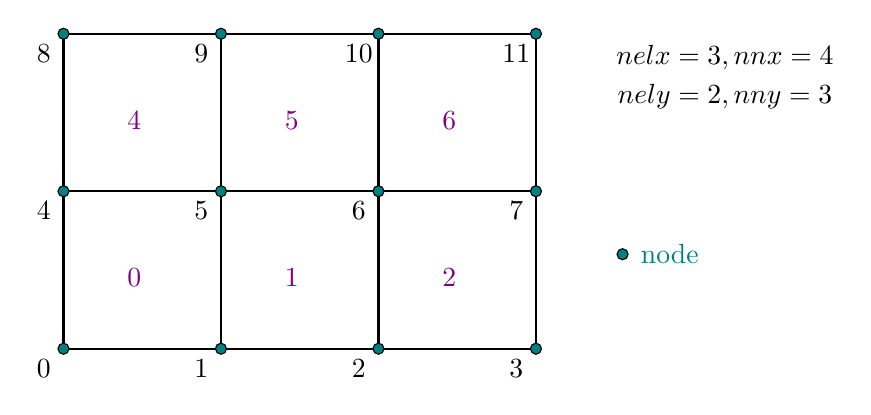
\begin{tikzpicture}
%\draw[step=0.5cm,gray,very thin] (0,0) grid (9,5); %background grid

\draw[thick] (1,1) -- (7,1) -- (7,5) -- (1,5) -- cycle;  
\draw[thick] (1,3) -- (7,3) ;
\draw[thick] (3,1) -- (3,5) ;
\draw[thick] (5,1) -- (5,5) ;

\draw[black,fill=teal] (1,1)     circle (2pt); 
\draw[black,fill=teal] (3,1)     circle (2pt); 
\draw[black,fill=teal] (5,1)     circle (2pt); 
\draw[black,fill=teal] (7,1)     circle (2pt); 

\draw[black,fill=teal] (1,3)     circle (2pt); 
\draw[black,fill=teal] (3,3)     circle (2pt); 
\draw[black,fill=teal] (5,3)     circle (2pt); 
\draw[black,fill=teal] (7,3)     circle (2pt); 

\draw[black,fill=teal] (1,5)     circle (2pt); 
\draw[black,fill=teal] (3,5)     circle (2pt); 
\draw[black,fill=teal] (5,5)     circle (2pt); 
\draw[black,fill=teal] (7,5)     circle (2pt); 

\node[] at (0.75,0.75) {0};
\node[] at (2.75,0.75) {1};
\node[] at (4.75,0.75) {2};
\node[] at (6.75,0.75) {3};

\node[] at (0.75,2.75) {4};
\node[] at (2.75,2.75) {5};
\node[] at (4.75,2.75) {6};
\node[] at (6.75,2.75) {7};

\node[] at (0.75,4.75) {8};
\node[] at (2.75,4.75) {9};
\node[] at (4.75,4.75) {10};
\node[] at (6.75,4.75) {11};

\node[violet] at (1.9,1.9) {0};
\node[violet] at (3.9,1.9) {1};
\node[violet] at (5.9,1.9) {2};
\node[violet] at (1.9,3.9) {4};
\node[violet] at (3.9,3.9) {5};
\node[violet] at (5.9,3.9) {6};

\draw[black,fill=teal] (8.1,2.2) circle (2pt); 
\node[] at (8.7,2.2) {{\color{teal}node}};

\node[] at (9.4,4.7) {$nelx=3, nnx=4$};
\node[] at (9.4,4.2) {$nely=2, nny=3$};

\end{tikzpicture}

\end{center}

\noindent In the case there is only a single degree of freedom per node, the 
assembled FEM matrix ${\bm M}$ will look like this:
\[
{\bm M}=
\left(
\begin{array}{cccccccccccc}
\Box & \Box &      &      & \Box & \Box &      &      &      &      &      &      \\
\Box & \Box & \Box &      & \Box & \Box & \Box &      &      &      &      &      \\
     & \Box & \Box & \Box &      & \Box & \Box & \Box &      &      &      &      \\
     &      & \Box & \Box &      &      & \Box & \Box &      &      &      &      \\
\Box & \Box &      &      & \Box & \Box &      &      & \Box & \Box &      &      \\
\Box & \Box & \Box &      & \Box & \Box & \Box &      & \Box & \Box & \Box &      \\
     & \Box & \Box & \Box &      & \Box & \Box & \Box &      & \Box & \Box & \Box \\
     &      & \Box & \Box &      &      & \Box & \Box &      &      & \Box & \Box \\
     &      &      &      & \Box & \Box &      &      & \Box & \Box &      &      \\
     &      &      &      & \Box & \Box & \Box &      & \Box & \Box & \Box &      \\
     &      &      &      &      & \Box & \Box & \Box &      & \Box & \Box & \Box \\
     &      &      &      &      &      & \Box & \Box &      &      & \Box & \Box 
\end{array}
\right)
\]
where the $\Box$ stand for non-zero terms.
This matrix structure stems from the fact that
\begin{itemize}
\item node 0 sees nodes 0,1,4,5 (1st line/column of the matrix)
\item node 1 sees nodes 0,1,2,4,5,6 (2nd line/column of the matrix)
\item node 2 sees nodes 1,2,3,5,6,7 (3rd line/column of the matrix)
\item node 3 sees nodes 2,3,6,7
\item node 4 sees nodes 0,1,4,5,8,9
\item node 5 sees nodes 0,1,2,4,5,6,8,9,10 
\item node 6 sees nodes 1,2,3,5,6,7,9,10,11
\item node 7 sees nodes 2,3,6,7,10,11
\item node 8 sees nodes 4,5,8,9
\item node 9 sees nodes 4,5,6,8,9,10
\item node 10 sees nodes 5,6,7,9,10,11 
\item node 11 sees nodes 6,7,10,11 (last line/column of the matrix)
\end{itemize}
In light thereof, we have
\begin{itemize}
\item 4 corner nodes which have 4 neighbours (counting themselves) 
\item 2(nnx-2) nodes which have 6 neighbours
\item 2(nny-2) nodes which have 6 neighbours
\item (nnx-2)$\times$(nny-2) nodes which have 9 neighbours
\end{itemize}
In total, the number of non-zero terms in the matrix above is then:
\[
NZ=4\times4+4\times6+2\times6+2\times9=70
\]
and in general, we would then have:
\[
NZ=4\times4+[2(nnx-2)+2(nny-2)]\times6 + (nnx-2)(nny-2)\times9
\]
Let us temporarily assume $nnx=nny=n$. The matrix size (total
number of unknowns) is then $N=n^2$ and  
\[
NZ=16+24(n-2)+9(n-2)^2
\]
A full matrix array would contain $N^2=n^4$ terms. 
The ratio of $NZ$ (the actual number of reals to store)
to the full matrix size (the number of reals a full matrix contains) is then 
\[
R = \frac{16+24(n-2)+9(n-2)^2}{n^4}
\]
It is then obvious that when $n$ is large enough $R \sim 1/n^2$.

CSR stores the nonzeros of the matrix row by row, in a
single indexed array A of double precision  numbers.
Another array COLIND contains the column index of each
corresponding entry in the A array. A third integer array RWPTR
contains pointers to the beginning of each row, which an additional pointer to
the first index following the nonzeros of the matrix A.
A and COLIND have length NZ and RWPTR has length N+1.

In the case of the here-above matrix, the arrays COLIND and RWPTR will look like:
\begin{eqnarray}
COLIND&=&(0,1,4,5, \; 0,1,2,4,5,6, \; 1,2,3,5,6,7, ..., 6,7,10,11) \nn\\
RWPTR &=&(0,4,10,16, ... )   \nn
\end{eqnarray}


%..............................................................................
\subsubsection{2D domain - Symmetric matrix CSR storage} \label{ss:symmcsrss}

If the matrix is symmetric, i.e. ${\bm M}={\bm M}^T$, then we may wish to 
only store half of it, always in the interest of saving memory. 
Only the following remaining $\Box$ entries are relevant now:
\[
{\bm M}=
\left(
\begin{array}{cccccccccccc}
\Box & \Box &      &      & \Box & \Box &      &      &      &      &      &      \\
     & \Box & \Box &      & \Box & \Box & \Box &      &      &      &      &      \\
     &      & \Box & \Box &      & \Box & \Box & \Box &      &      &      &      \\
     &      &      & \Box &      &      & \Box & \Box &      &      &      &      \\
     &      &      &      & \Box & \Box &      &      & \Box & \Box &      &      \\
     &      &      &      &      & \Box & \Box &      & \Box & \Box & \Box &      \\
     &      &      &      &      &      & \Box & \Box &      & \Box & \Box & \Box \\
     &      &      &      &      &      &      & \Box &      &      & \Box & \Box \\
     &      &      &      &      &      &      &      & \Box & \Box &      &      \\
     &      &      &      &      &      &      &      &      & \Box & \Box &      \\
     &      &      &      &      &      &      &      &      &      & \Box & \Box \\
     &      &      &      &      &      &      &      &      &      &      & \Box 
\end{array}
\right)
\]
We see that the number of nonzeros is now 
\[
NZ_{symm}= \frac{NZ-n}{2}+n
\]
and in this case $NZ_{symm}=(70-12)/2+12=41$.
Then 
\begin{eqnarray}
COLIND&=&(0,1,4,5, \; 1,2,4,5,6, \; 3,5,6,7, ..., ,11) \nn\\
RWPTR &=&(0,4,9,14, ... )   \nn
\end{eqnarray}

In case the numbering is Fortran-like, then 
\begin{eqnarray}
ja=COLIND&=&(
1, 2, 5, 6, \quad  2, 3, 5, 6, 7, \quad 3, 4, 6, 7, 8, \quad      
4, 7, 8, \quad  5, 6, 9, 10, \quad 6, 7, 9, 10, 11, \nn\\
&& 7, 8, 10, 11, 12, \quad 8, 11, 12, \quad 9, 10, \quad 10, 11, \quad  11, 12, \quad 12) \nn\\
ia=RWPTR &=&(1, 5, 10, 15, 18, 22, 27, 32, 35, 37, 39, 41, 42)  \nn
\end{eqnarray}

%..............................................................................
\subsubsection{2D domain - Two degrees of freedom per node}

When there are now two degrees of freedom per node, such as in the case of the Stokes equation
in two-dimensions, the size of the $\K$ matrix is given $NfemV=nnx*nny*ndofV$  
where $NfemV$ is the total number of velocity degrees of freedom.

\begin{center}
\begin{flushright} {\tiny {\color{gray} (tikz\_3x2\_two.tex)}} \end{flushright}
%~~~~~~~~~~~~~~~~~~~~~~~~~~~~~~~~~~~~~~~~~~~~~~~~~~~~~~~~~~~~~~~~~~~~~~~~~~~~~~~~~~~~~~~~~~~~~~~~~~


\begin{tikzpicture}
%\draw[step=0.5cm,gray,very thin] (0,0) grid (5,5); %background grid

\draw[thick] (1,1) -- (7,1) -- (7,5) -- (1,5) -- cycle;  
\draw[thick] (1,3) -- (7,3) ;
\draw[thick] (3,1) -- (3,5) ;
\draw[thick] (5,1) -- (5,5) ;

\draw[black,fill=teal] (1,1)     circle (2pt); 
\draw[black,fill=teal] (3,1)     circle (2pt); 
\draw[black,fill=teal] (5,1)     circle (2pt); 
\draw[black,fill=teal] (7,1)     circle (2pt); 

\draw[black,fill=teal] (1,3)     circle (2pt); 
\draw[black,fill=teal] (3,3)     circle (2pt); 
\draw[black,fill=teal] (5,3)     circle (2pt); 
\draw[black,fill=teal] (7,3)     circle (2pt); 

\draw[black,fill=teal] (1,5)     circle (2pt); 
\draw[black,fill=teal] (3,5)     circle (2pt); 
\draw[black,fill=teal] (5,5)     circle (2pt); 
\draw[black,fill=teal] (7,5)     circle (2pt); 

\node[] at (0.75,0.7) {0,1};
\node[] at (2.75,0.7) {2,3};
\node[] at (4.75,0.7) {4,5};
\node[] at (6.75,0.7) {6,7};

\node[] at (0.65,2.7) {8,9};
\node[] at (2.475,2.7) {10,11};
\node[] at (4.475,2.7) {12,13};
\node[] at (6.475,2.7) {14,15};

\node[] at (0.475,4.7) {16,17};
\node[] at (2.475,4.7) {18,19};
\node[] at (4.475,4.7) {20,21};
\node[] at (6.475,4.7) {22,23};

\node[violet] at (1.9,1.9) {0};
\node[violet] at (3.9,1.9) {1};
\node[violet] at (5.9,1.9) {2};
\node[violet] at (1.9,3.9) {4};
\node[violet] at (3.9,3.9) {5};
\node[violet] at (5.9,3.9) {6};

\draw[black,fill=teal] (8.1,2.2) circle (2pt); 
\node[] at (8.4,2.2) {$\vec\upnu$};

\end{tikzpicture}





\end{center}

In the case of the small grid above, we have then $NfemV=24$ and
elemental matrices are now $8\times8$ in size.

We still have
\begin{itemize}
\item $4$ corner nodes which have 4 neighbours
\item $2(nnx-2)$ nodes which have 6 neighbours
\item $2(nny-2)$ nodes which have 6 neighbours
\item $(nnx-2)\cdot(nny-2)$ nodes which have 9 neighbours,
\end{itemize}
but now each degree of freedom from a node sees the other two
degrees of freedom of another node too.
In that case, the number of nonzeros has been multiplied by four
and the assembled FEM matrix looks like:
\begin{equation}
\left(
\begin{array}{cccccccccccccccccccccccc}
\Box&\Box & \Box&\Box &  &  &  &  & \Box&\Box & \Box&\Box &  &  &  &  &  &  &  &  &  &  &  &  \\
\Box&\Box & \Box&\Box &  &  &  &  & \Box&\Box & \Box&\Box &  &  &  &  &  &  &  &  &  &  &  &  \\
\Box&\Box & \Box&\Box & \Box&\Box &  &  & \Box&\Box & \Box&\Box & \Box&\Box &  &  &  &  &  &  &  &  &  &  \\
\Box&\Box & \Box&\Box & \Box&\Box &  &  & \Box&\Box & \Box&\Box & \Box&\Box &  &  &  &  &  &  &  &  &  &  \\
 &  & \Box&\Box & \Box&\Box & \Box&\Box &  &  & \Box&\Box & \Box&\Box & \Box&\Box &  &  &  &  &  &  &  &  \\
 &  & \Box&\Box & \Box&\Box & \Box&\Box &  &  & \Box&\Box & \Box&\Box & \Box&\Box &  &  &  &  &  &  &  &  \\
 &  &  &  & \Box&\Box & \Box&\Box &  &  &  &  & \Box&\Box & \Box&\Box &  &  &  &  &  &  &  &  \\
 &  &  &  & \Box&\Box & \Box&\Box &  &  &  &  & \Box&\Box & \Box&\Box &  &  &  &  &  &  &  &  \\
\Box&\Box & \Box&\Box &  &  &  &  & \Box&\Box & \Box&\Box &  &  &  &  & \Box&\Box & \Box&\Box &  &  &  &  \\
\Box&\Box & \Box&\Box &  &  &  &  & \Box&\Box & \Box&\Box &  &  &  &  & \Box&\Box & \Box&\Box &  &  &  &  \\
\Box&\Box & \Box&\Box & \Box&\Box &  &  & \Box&\Box & \Box&\Box & \Box&\Box &  &  & \Box&\Box & \Box&\Box & \Box&\Box &  &  \\
\Box&\Box & \Box&\Box & \Box&\Box &  &  & \Box&\Box & \Box&\Box & \Box&\Box &  &  & \Box&\Box & \Box&\Box & \Box&\Box &  &  \\
 &  & \Box&\Box & \Box&\Box & \Box&\Box &  &  & \Box&\Box & \Box&\Box & \Box&\Box &  &  & \Box&\Box & \Box&\Box & \Box&\Box \\
 &  & \Box&\Box & \Box&\Box & \Box&\Box &  &  & \Box&\Box & \Box&\Box & \Box&\Box &  &  & \Box&\Box & \Box&\Box & \Box&\Box \\
 &  &  &  & \Box&\Box & \Box&\Box &  &  &  &  & \Box&\Box & \Box&\Box &  &  &  &  & \Box&\Box & \Box&\Box \\
 &  &  &  & \Box&\Box & \Box&\Box &  &  &  &  & \Box&\Box & \Box&\Box &  &  &  &  & \Box&\Box & \Box&\Box \\
 &  &  &  &  &  &  &  & \Box&\Box & \Box&\Box &  &  &  &  & \Box&\Box & \Box&\Box &  &  &  &  \\
 &  &  &  &  &  &  &  & \Box&\Box & \Box&\Box &  &  &  &  & \Box&\Box & \Box&\Box &  &  &  &  \\
 &  &  &  &  &  &  &  & \Box&\Box & \Box&\Box & \Box&\Box &  &  & \Box&\Box & \Box&\Box & \Box&\Box &  &  \\
 &  &  &  &  &  &  &  & \Box&\Box & \Box&\Box & \Box&\Box &  &  & \Box&\Box & \Box&\Box & \Box&\Box &  &  \\
 &  &  &  &  &  &  &  &  &  & \Box&\Box & \Box&\Box & \Box&\Box &  &  & \Box&\Box & \Box&\Box & \Box&\Box \\
 &  &  &  &  &  &  &  &  &  & \Box&\Box & \Box&\Box & \Box&\Box &  &  & \Box&\Box & \Box&\Box & \Box&\Box \\
 &  &  &  &  &  &  &  &  &  &  &  & \Box&\Box & \Box&\Box &  &  &  &  & \Box&\Box & \Box&\Box \\
 &  &  &  &  &  &  &  &  &  &  &  & \Box&\Box & \Box&\Box &  &  &  &  & \Box&\Box & \Box&\Box 
\end{array}
\right)\nonumber
\end{equation}
Note that the degrees of freedom are organised as follows: 
\[
(u_0,v_0,u_1,v_1,u_2,v_2, ... u_{11},v_{11})
\]
In general, we would then have:
\[
NZ=4 \left[4\times4+[2(nnx-2)+2(nny-2)]\times6 + (nnx-2)(nny-2)\times9 \right]
\]
and in the case of the small grid,
the number of non-zero terms in the matrix is then:
\[
NZ=4\left[4\times4+4\times6+2\times6+2\times9\right]=280
\]
In the case of the here-above matrix, the arrays COLIND and RWPTR will look like:
\begin{eqnarray}
COLIND&=&(0,1,2,3,8,9,10,11, \; 0,1,2,3,8,9,10,11,\; ...) \nn\\
RWPTR &=&(0,8,16,28, ... ) \nn
\end{eqnarray}

Assuming we are using $Q_1\times P_0$ elements, the structure of the matrix $\G_{el}^T$ is as follows
(the 6 pressure dofs are connected to 24 velocity dofs):

\begin{scriptsize}
\begin{equation}
\left(
\begin{array}{ccccccccccccccccccccccccc}
&0 & 1 & 2 & 3 & 4 & 5 & 6 & 7 & 8 & 9 & 10 & 11 & 12 & 13 & 14 & 15 & 16 & 17 & 18 & 19 & 20 & 21 & 22 & 23     \\
\Box&\Box & \Box&\Box &  &  &  &  & \Box&\Box & \Box&\Box &  &  &  &  &  &  &  &  &  &  &  &  \\
    &     & \Box&\Box & \Box&\Box &  &  &  &  & \Box&\Box & \Box&\Box &  &  &  &  &  &  &  &  &  &  \\
 & &     &     & \Box&\Box & \Box&\Box &  &  &  &  & \Box&\Box & \Box&\Box &  &  &  &  &  &  &  &    \\
 & & & &  & &     &     & \Box&\Box & \Box&\Box &  &  &  &  & \Box&\Box & \Box&\Box &  &  &  &      \\
 & & & & & &  & &     &     & \Box&\Box & \Box&\Box &  &  &  &  & \Box&\Box & \Box&\Box &  &       \\
 & &  & & & & & &  & &     &     & \Box&\Box & \Box&\Box &  &  &  &  & \Box&\Box & \Box&\Box        
\end{array}
\right)
\end{equation} 
\end{scriptsize}

\begin{center}
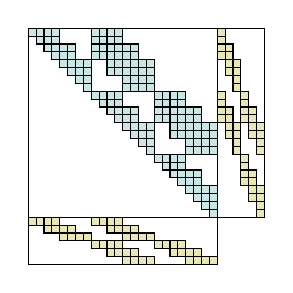
\begin{tikzpicture}
\draw[] (   0.1,   0.7) rectangle (   2.5,   3.1);
\draw[fill=teal!20] (   0.1,   3.0) rectangle (   0.2,   3.1);
\draw[fill=teal!20] (   0.2,   3.0) rectangle (   0.3,   3.1);
\draw[fill=teal!20] (   0.3,   3.0) rectangle (   0.4,   3.1);
\draw[fill=teal!20] (   0.4,   3.0) rectangle (   0.5,   3.1);
\draw[fill=teal!20] (   0.9,   3.0) rectangle (   1.0,   3.1);
\draw[fill=teal!20] (   1.0,   3.0) rectangle (   1.1,   3.1);
\draw[fill=teal!20] (   1.1,   3.0) rectangle (   1.2,   3.1);
\draw[fill=teal!20] (   1.2,   3.0) rectangle (   1.3,   3.1);
\draw[fill=teal!20] (   0.2,   2.9) rectangle (   0.3,   3.0);
\draw[fill=teal!20] (   0.3,   2.9) rectangle (   0.4,   3.0);
\draw[fill=teal!20] (   0.4,   2.9) rectangle (   0.5,   3.0);
\draw[fill=teal!20] (   0.9,   2.9) rectangle (   1.0,   3.0);
\draw[fill=teal!20] (   1.0,   2.9) rectangle (   1.1,   3.0);
\draw[fill=teal!20] (   1.1,   2.9) rectangle (   1.2,   3.0);
\draw[fill=teal!20] (   1.2,   2.9) rectangle (   1.3,   3.0);
\draw[fill=teal!20] (   0.3,   2.8) rectangle (   0.4,   2.9);
\draw[fill=teal!20] (   0.4,   2.8) rectangle (   0.5,   2.9);
\draw[fill=teal!20] (   0.5,   2.8) rectangle (   0.6,   2.9);
\draw[fill=teal!20] (   0.6,   2.8) rectangle (   0.7,   2.9);
\draw[fill=teal!20] (   0.9,   2.8) rectangle (   1.0,   2.9);
\draw[fill=teal!20] (   1.0,   2.8) rectangle (   1.1,   2.9);
\draw[fill=teal!20] (   1.1,   2.8) rectangle (   1.2,   2.9);
\draw[fill=teal!20] (   1.2,   2.8) rectangle (   1.3,   2.9);
\draw[fill=teal!20] (   1.3,   2.8) rectangle (   1.4,   2.9);
\draw[fill=teal!20] (   1.4,   2.8) rectangle (   1.5,   2.9);
\draw[fill=teal!20] (   0.4,   2.7) rectangle (   0.5,   2.8);
\draw[fill=teal!20] (   0.5,   2.7) rectangle (   0.6,   2.8);
\draw[fill=teal!20] (   0.6,   2.7) rectangle (   0.7,   2.8);
\draw[fill=teal!20] (   0.9,   2.7) rectangle (   1.0,   2.8);
\draw[fill=teal!20] (   1.0,   2.7) rectangle (   1.1,   2.8);
\draw[fill=teal!20] (   1.1,   2.7) rectangle (   1.2,   2.8);
\draw[fill=teal!20] (   1.2,   2.7) rectangle (   1.3,   2.8);
\draw[fill=teal!20] (   1.3,   2.7) rectangle (   1.4,   2.8);
\draw[fill=teal!20] (   1.4,   2.7) rectangle (   1.5,   2.8);
\draw[fill=teal!20] (   0.5,   2.6) rectangle (   0.6,   2.7);
\draw[fill=teal!20] (   0.6,   2.6) rectangle (   0.7,   2.7);
\draw[fill=teal!20] (   0.7,   2.6) rectangle (   0.8,   2.7);
\draw[fill=teal!20] (   0.8,   2.6) rectangle (   0.9,   2.7);
\draw[fill=teal!20] (   1.1,   2.6) rectangle (   1.2,   2.7);
\draw[fill=teal!20] (   1.2,   2.6) rectangle (   1.3,   2.7);
\draw[fill=teal!20] (   1.3,   2.6) rectangle (   1.4,   2.7);
\draw[fill=teal!20] (   1.4,   2.6) rectangle (   1.5,   2.7);
\draw[fill=teal!20] (   1.5,   2.6) rectangle (   1.6,   2.7);
\draw[fill=teal!20] (   1.6,   2.6) rectangle (   1.7,   2.7);
\draw[fill=teal!20] (   0.6,   2.5) rectangle (   0.7,   2.6);
\draw[fill=teal!20] (   0.7,   2.5) rectangle (   0.8,   2.6);
\draw[fill=teal!20] (   0.8,   2.5) rectangle (   0.9,   2.6);
\draw[fill=teal!20] (   1.1,   2.5) rectangle (   1.2,   2.6);
\draw[fill=teal!20] (   1.2,   2.5) rectangle (   1.3,   2.6);
\draw[fill=teal!20] (   1.3,   2.5) rectangle (   1.4,   2.6);
\draw[fill=teal!20] (   1.4,   2.5) rectangle (   1.5,   2.6);
\draw[fill=teal!20] (   1.5,   2.5) rectangle (   1.6,   2.6);
\draw[fill=teal!20] (   1.6,   2.5) rectangle (   1.7,   2.6);
\draw[fill=teal!20] (   0.7,   2.4) rectangle (   0.8,   2.5);
\draw[fill=teal!20] (   0.8,   2.4) rectangle (   0.9,   2.5);
\draw[fill=teal!20] (   1.3,   2.4) rectangle (   1.4,   2.5);
\draw[fill=teal!20] (   1.4,   2.4) rectangle (   1.5,   2.5);
\draw[fill=teal!20] (   1.5,   2.4) rectangle (   1.6,   2.5);
\draw[fill=teal!20] (   1.6,   2.4) rectangle (   1.7,   2.5);
\draw[fill=teal!20] (   0.8,   2.3) rectangle (   0.9,   2.4);
\draw[fill=teal!20] (   1.3,   2.3) rectangle (   1.4,   2.4);
\draw[fill=teal!20] (   1.4,   2.3) rectangle (   1.5,   2.4);
\draw[fill=teal!20] (   1.5,   2.3) rectangle (   1.6,   2.4);
\draw[fill=teal!20] (   1.6,   2.3) rectangle (   1.7,   2.4);
\draw[fill=teal!20] (   0.9,   2.2) rectangle (   1.0,   2.3);
\draw[fill=teal!20] (   1.0,   2.2) rectangle (   1.1,   2.3);
\draw[fill=teal!20] (   1.1,   2.2) rectangle (   1.2,   2.3);
\draw[fill=teal!20] (   1.2,   2.2) rectangle (   1.3,   2.3);
\draw[fill=teal!20] (   1.7,   2.2) rectangle (   1.8,   2.3);
\draw[fill=teal!20] (   1.8,   2.2) rectangle (   1.9,   2.3);
\draw[fill=teal!20] (   1.9,   2.2) rectangle (   2.0,   2.3);
\draw[fill=teal!20] (   2.0,   2.2) rectangle (   2.1,   2.3);
\draw[fill=teal!20] (   1.0,   2.1) rectangle (   1.1,   2.2);
\draw[fill=teal!20] (   1.1,   2.1) rectangle (   1.2,   2.2);
\draw[fill=teal!20] (   1.2,   2.1) rectangle (   1.3,   2.2);
\draw[fill=teal!20] (   1.7,   2.1) rectangle (   1.8,   2.2);
\draw[fill=teal!20] (   1.8,   2.1) rectangle (   1.9,   2.2);
\draw[fill=teal!20] (   1.9,   2.1) rectangle (   2.0,   2.2);
\draw[fill=teal!20] (   2.0,   2.1) rectangle (   2.1,   2.2);
\draw[fill=teal!20] (   1.1,   2.0) rectangle (   1.2,   2.1);
\draw[fill=teal!20] (   1.2,   2.0) rectangle (   1.3,   2.1);
\draw[fill=teal!20] (   1.3,   2.0) rectangle (   1.4,   2.1);
\draw[fill=teal!20] (   1.4,   2.0) rectangle (   1.5,   2.1);
\draw[fill=teal!20] (   1.7,   2.0) rectangle (   1.8,   2.1);
\draw[fill=teal!20] (   1.8,   2.0) rectangle (   1.9,   2.1);
\draw[fill=teal!20] (   1.9,   2.0) rectangle (   2.0,   2.1);
\draw[fill=teal!20] (   2.0,   2.0) rectangle (   2.1,   2.1);
\draw[fill=teal!20] (   2.1,   2.0) rectangle (   2.2,   2.1);
\draw[fill=teal!20] (   2.2,   2.0) rectangle (   2.3,   2.1);
\draw[fill=teal!20] (   1.2,   1.9) rectangle (   1.3,   2.0);
\draw[fill=teal!20] (   1.3,   1.9) rectangle (   1.4,   2.0);
\draw[fill=teal!20] (   1.4,   1.9) rectangle (   1.5,   2.0);
\draw[fill=teal!20] (   1.7,   1.9) rectangle (   1.8,   2.0);
\draw[fill=teal!20] (   1.8,   1.9) rectangle (   1.9,   2.0);
\draw[fill=teal!20] (   1.9,   1.9) rectangle (   2.0,   2.0);
\draw[fill=teal!20] (   2.0,   1.9) rectangle (   2.1,   2.0);
\draw[fill=teal!20] (   2.1,   1.9) rectangle (   2.2,   2.0);
\draw[fill=teal!20] (   2.2,   1.9) rectangle (   2.3,   2.0);
\draw[fill=teal!20] (   1.3,   1.8) rectangle (   1.4,   1.9);
\draw[fill=teal!20] (   1.4,   1.8) rectangle (   1.5,   1.9);
\draw[fill=teal!20] (   1.5,   1.8) rectangle (   1.6,   1.9);
\draw[fill=teal!20] (   1.6,   1.8) rectangle (   1.7,   1.9);
\draw[fill=teal!20] (   1.9,   1.8) rectangle (   2.0,   1.9);
\draw[fill=teal!20] (   2.0,   1.8) rectangle (   2.1,   1.9);
\draw[fill=teal!20] (   2.1,   1.8) rectangle (   2.2,   1.9);
\draw[fill=teal!20] (   2.2,   1.8) rectangle (   2.3,   1.9);
\draw[fill=teal!20] (   2.3,   1.8) rectangle (   2.4,   1.9);
\draw[fill=teal!20] (   2.4,   1.8) rectangle (   2.5,   1.9);
\draw[fill=teal!20] (   1.4,   1.7) rectangle (   1.5,   1.8);
\draw[fill=teal!20] (   1.5,   1.7) rectangle (   1.6,   1.8);
\draw[fill=teal!20] (   1.6,   1.7) rectangle (   1.7,   1.8);
\draw[fill=teal!20] (   1.9,   1.7) rectangle (   2.0,   1.8);
\draw[fill=teal!20] (   2.0,   1.7) rectangle (   2.1,   1.8);
\draw[fill=teal!20] (   2.1,   1.7) rectangle (   2.2,   1.8);
\draw[fill=teal!20] (   2.2,   1.7) rectangle (   2.3,   1.8);
\draw[fill=teal!20] (   2.3,   1.7) rectangle (   2.4,   1.8);
\draw[fill=teal!20] (   2.4,   1.7) rectangle (   2.5,   1.8);
\draw[fill=teal!20] (   1.5,   1.6) rectangle (   1.6,   1.7);
\draw[fill=teal!20] (   1.6,   1.6) rectangle (   1.7,   1.7);
\draw[fill=teal!20] (   2.1,   1.6) rectangle (   2.2,   1.7);
\draw[fill=teal!20] (   2.2,   1.6) rectangle (   2.3,   1.7);
\draw[fill=teal!20] (   2.3,   1.6) rectangle (   2.4,   1.7);
\draw[fill=teal!20] (   2.4,   1.6) rectangle (   2.5,   1.7);
\draw[fill=teal!20] (   1.6,   1.5) rectangle (   1.7,   1.6);
\draw[fill=teal!20] (   2.1,   1.5) rectangle (   2.2,   1.6);
\draw[fill=teal!20] (   2.2,   1.5) rectangle (   2.3,   1.6);
\draw[fill=teal!20] (   2.3,   1.5) rectangle (   2.4,   1.6);
\draw[fill=teal!20] (   2.4,   1.5) rectangle (   2.5,   1.6);
\draw[fill=teal!20] (   1.7,   1.4) rectangle (   1.8,   1.5);
\draw[fill=teal!20] (   1.8,   1.4) rectangle (   1.9,   1.5);
\draw[fill=teal!20] (   1.9,   1.4) rectangle (   2.0,   1.5);
\draw[fill=teal!20] (   2.0,   1.4) rectangle (   2.1,   1.5);
\draw[fill=teal!20] (   1.8,   1.3) rectangle (   1.9,   1.4);
\draw[fill=teal!20] (   1.9,   1.3) rectangle (   2.0,   1.4);
\draw[fill=teal!20] (   2.0,   1.3) rectangle (   2.1,   1.4);
\draw[fill=teal!20] (   1.9,   1.2) rectangle (   2.0,   1.3);
\draw[fill=teal!20] (   2.0,   1.2) rectangle (   2.1,   1.3);
\draw[fill=teal!20] (   2.1,   1.2) rectangle (   2.2,   1.3);
\draw[fill=teal!20] (   2.2,   1.2) rectangle (   2.3,   1.3);
\draw[fill=teal!20] (   2.0,   1.1) rectangle (   2.1,   1.2);
\draw[fill=teal!20] (   2.1,   1.1) rectangle (   2.2,   1.2);
\draw[fill=teal!20] (   2.2,   1.1) rectangle (   2.3,   1.2);
\draw[fill=teal!20] (   2.1,   1.0) rectangle (   2.2,   1.1);
\draw[fill=teal!20] (   2.2,   1.0) rectangle (   2.3,   1.1);
\draw[fill=teal!20] (   2.3,   1.0) rectangle (   2.4,   1.1);
\draw[fill=teal!20] (   2.4,   1.0) rectangle (   2.5,   1.1);
\draw[fill=teal!20] (   2.2,   0.9) rectangle (   2.3,   1.0);
\draw[fill=teal!20] (   2.3,   0.9) rectangle (   2.4,   1.0);
\draw[fill=teal!20] (   2.4,   0.9) rectangle (   2.5,   1.0);
\draw[fill=teal!20] (   2.3,   0.8) rectangle (   2.4,   0.9);
\draw[fill=teal!20] (   2.4,   0.8) rectangle (   2.5,   0.9);
\draw[fill=teal!20] (   2.4,   0.7) rectangle (   2.5,   0.8);
\draw[] (   2.5,   0.7) rectangle (   3.1,   3.1);
\draw[fill=olive!20] (   3.0,   0.7) rectangle (   3.1,   0.8);
\draw[fill=olive!20] (   3.0,   0.8) rectangle (   3.1,   0.9);
\draw[fill=olive!20] (   3.0,   0.9) rectangle (   3.1,   1.0);
\draw[fill=olive!20] (   3.0,   1.0) rectangle (   3.1,   1.1);
\draw[fill=olive!20] (   3.0,   1.7) rectangle (   3.1,   1.8);
\draw[fill=olive!20] (   3.0,   1.8) rectangle (   3.1,   1.9);
\draw[fill=olive!20] (   3.0,   1.5) rectangle (   3.1,   1.6);
\draw[fill=olive!20] (   3.0,   1.6) rectangle (   3.1,   1.7);
\draw[fill=olive!20] (   2.9,   0.9) rectangle (   3.0,   1.0);
\draw[fill=olive!20] (   2.9,   1.0) rectangle (   3.0,   1.1);
\draw[fill=olive!20] (   2.9,   1.1) rectangle (   3.0,   1.2);
\draw[fill=olive!20] (   2.9,   1.2) rectangle (   3.0,   1.3);
\draw[fill=olive!20] (   2.9,   1.9) rectangle (   3.0,   2.0);
\draw[fill=olive!20] (   2.9,   2.0) rectangle (   3.0,   2.1);
\draw[fill=olive!20] (   2.9,   1.7) rectangle (   3.0,   1.8);
\draw[fill=olive!20] (   2.9,   1.8) rectangle (   3.0,   1.9);
\draw[fill=olive!20] (   2.8,   1.1) rectangle (   2.9,   1.2);
\draw[fill=olive!20] (   2.8,   1.2) rectangle (   2.9,   1.3);
\draw[fill=olive!20] (   2.8,   1.3) rectangle (   2.9,   1.4);
\draw[fill=olive!20] (   2.8,   1.4) rectangle (   2.9,   1.5);
\draw[fill=olive!20] (   2.8,   2.1) rectangle (   2.9,   2.2);
\draw[fill=olive!20] (   2.8,   2.2) rectangle (   2.9,   2.3);
\draw[fill=olive!20] (   2.8,   1.9) rectangle (   2.9,   2.0);
\draw[fill=olive!20] (   2.8,   2.0) rectangle (   2.9,   2.1);
\draw[fill=olive!20] (   2.7,   1.5) rectangle (   2.8,   1.6);
\draw[fill=olive!20] (   2.7,   1.6) rectangle (   2.8,   1.7);
\draw[fill=olive!20] (   2.7,   1.7) rectangle (   2.8,   1.8);
\draw[fill=olive!20] (   2.7,   1.8) rectangle (   2.8,   1.9);
\draw[fill=olive!20] (   2.7,   2.5) rectangle (   2.8,   2.6);
\draw[fill=olive!20] (   2.7,   2.6) rectangle (   2.8,   2.7);
\draw[fill=olive!20] (   2.7,   2.3) rectangle (   2.8,   2.4);
\draw[fill=olive!20] (   2.7,   2.4) rectangle (   2.8,   2.5);
\draw[fill=olive!20] (   2.6,   1.7) rectangle (   2.7,   1.8);
\draw[fill=olive!20] (   2.6,   1.8) rectangle (   2.7,   1.9);
\draw[fill=olive!20] (   2.6,   1.9) rectangle (   2.7,   2.0);
\draw[fill=olive!20] (   2.6,   2.0) rectangle (   2.7,   2.1);
\draw[fill=olive!20] (   2.6,   2.7) rectangle (   2.7,   2.8);
\draw[fill=olive!20] (   2.6,   2.8) rectangle (   2.7,   2.9);
\draw[fill=olive!20] (   2.6,   2.5) rectangle (   2.7,   2.6);
\draw[fill=olive!20] (   2.6,   2.6) rectangle (   2.7,   2.7);
\draw[fill=olive!20] (   2.5,   1.9) rectangle (   2.6,   2.0);
\draw[fill=olive!20] (   2.5,   2.0) rectangle (   2.6,   2.1);
\draw[fill=olive!20] (   2.5,   2.1) rectangle (   2.6,   2.2);
\draw[fill=olive!20] (   2.5,   2.2) rectangle (   2.6,   2.3);
\draw[fill=olive!20] (   2.5,   2.9) rectangle (   2.6,   3.0);
\draw[fill=olive!20] (   2.5,   3.0) rectangle (   2.6,   3.1);
\draw[fill=olive!20] (   2.5,   2.7) rectangle (   2.6,   2.8);
\draw[fill=olive!20] (   2.5,   2.8) rectangle (   2.6,   2.9);
\draw[] (   0.1,   0.1) rectangle (   2.5,   0.7);
\draw[fill=olive!20] (   0.1,   0.6) rectangle (   0.2,   0.7);
\draw[fill=olive!20] (   0.2,   0.6) rectangle (   0.3,   0.7);
\draw[fill=olive!20] (   0.3,   0.6) rectangle (   0.4,   0.7);
\draw[fill=olive!20] (   0.4,   0.6) rectangle (   0.5,   0.7);
\draw[fill=olive!20] (   1.1,   0.6) rectangle (   1.2,   0.7);
\draw[fill=olive!20] (   1.2,   0.6) rectangle (   1.3,   0.7);
\draw[fill=olive!20] (   0.9,   0.6) rectangle (   1.0,   0.7);
\draw[fill=olive!20] (   1.0,   0.6) rectangle (   1.1,   0.7);
\draw[fill=olive!20] (   0.3,   0.5) rectangle (   0.4,   0.6);
\draw[fill=olive!20] (   0.4,   0.5) rectangle (   0.5,   0.6);
\draw[fill=olive!20] (   0.5,   0.5) rectangle (   0.6,   0.6);
\draw[fill=olive!20] (   0.6,   0.5) rectangle (   0.7,   0.6);
\draw[fill=olive!20] (   1.3,   0.5) rectangle (   1.4,   0.6);
\draw[fill=olive!20] (   1.4,   0.5) rectangle (   1.5,   0.6);
\draw[fill=olive!20] (   1.1,   0.5) rectangle (   1.2,   0.6);
\draw[fill=olive!20] (   1.2,   0.5) rectangle (   1.3,   0.6);
\draw[fill=olive!20] (   0.5,   0.4) rectangle (   0.6,   0.5);
\draw[fill=olive!20] (   0.6,   0.4) rectangle (   0.7,   0.5);
\draw[fill=olive!20] (   0.7,   0.4) rectangle (   0.8,   0.5);
\draw[fill=olive!20] (   0.8,   0.4) rectangle (   0.9,   0.5);
\draw[fill=olive!20] (   1.5,   0.4) rectangle (   1.6,   0.5);
\draw[fill=olive!20] (   1.6,   0.4) rectangle (   1.7,   0.5);
\draw[fill=olive!20] (   1.3,   0.4) rectangle (   1.4,   0.5);
\draw[fill=olive!20] (   1.4,   0.4) rectangle (   1.5,   0.5);
\draw[fill=olive!20] (   0.9,   0.3) rectangle (   1.0,   0.4);
\draw[fill=olive!20] (   1.0,   0.3) rectangle (   1.1,   0.4);
\draw[fill=olive!20] (   1.1,   0.3) rectangle (   1.2,   0.4);
\draw[fill=olive!20] (   1.2,   0.3) rectangle (   1.3,   0.4);
\draw[fill=olive!20] (   1.9,   0.3) rectangle (   2.0,   0.4);
\draw[fill=olive!20] (   2.0,   0.3) rectangle (   2.1,   0.4);
\draw[fill=olive!20] (   1.7,   0.3) rectangle (   1.8,   0.4);
\draw[fill=olive!20] (   1.8,   0.3) rectangle (   1.9,   0.4);
\draw[fill=olive!20] (   1.1,   0.2) rectangle (   1.2,   0.3);
\draw[fill=olive!20] (   1.2,   0.2) rectangle (   1.3,   0.3);
\draw[fill=olive!20] (   1.3,   0.2) rectangle (   1.4,   0.3);
\draw[fill=olive!20] (   1.4,   0.2) rectangle (   1.5,   0.3);
\draw[fill=olive!20] (   2.1,   0.2) rectangle (   2.2,   0.3);
\draw[fill=olive!20] (   2.2,   0.2) rectangle (   2.3,   0.3);
\draw[fill=olive!20] (   1.9,   0.2) rectangle (   2.0,   0.3);
\draw[fill=olive!20] (   2.0,   0.2) rectangle (   2.1,   0.3);
\draw[fill=olive!20] (   1.3,   0.1) rectangle (   1.4,   0.2);
\draw[fill=olive!20] (   1.4,   0.1) rectangle (   1.5,   0.2);
\draw[fill=olive!20] (   1.5,   0.1) rectangle (   1.6,   0.2);
\draw[fill=olive!20] (   1.6,   0.1) rectangle (   1.7,   0.2);
\draw[fill=olive!20] (   2.3,   0.1) rectangle (   2.4,   0.2);
\draw[fill=olive!20] (   2.4,   0.1) rectangle (   2.5,   0.2);
\draw[fill=olive!20] (   2.1,   0.1) rectangle (   2.2,   0.2);
\draw[fill=olive!20] (   2.2,   0.1) rectangle (   2.3,   0.2);
\end{tikzpicture}

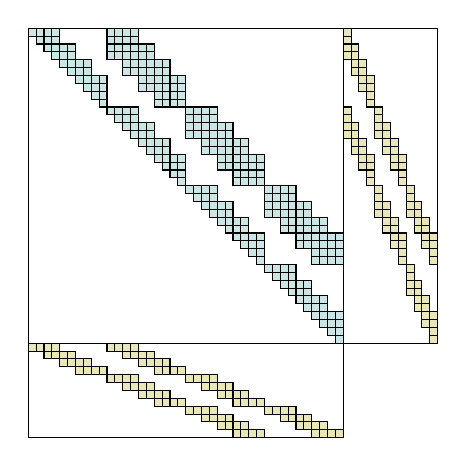
\begin{tikzpicture}
\draw[] (   0.1,   1.3) rectangle (   4.1,   5.3);
\draw[fill=teal!20] (   0.1,   5.2) rectangle (   0.2,   5.3);
\draw[fill=teal!20] (   0.2,   5.2) rectangle (   0.3,   5.3);
\draw[fill=teal!20] (   0.3,   5.2) rectangle (   0.4,   5.3);
\draw[fill=teal!20] (   0.4,   5.2) rectangle (   0.5,   5.3);
\draw[fill=teal!20] (   1.1,   5.2) rectangle (   1.2,   5.3);
\draw[fill=teal!20] (   1.2,   5.2) rectangle (   1.3,   5.3);
\draw[fill=teal!20] (   1.3,   5.2) rectangle (   1.4,   5.3);
\draw[fill=teal!20] (   1.4,   5.2) rectangle (   1.5,   5.3);
\draw[fill=teal!20] (   0.2,   5.1) rectangle (   0.3,   5.2);
\draw[fill=teal!20] (   0.3,   5.1) rectangle (   0.4,   5.2);
\draw[fill=teal!20] (   0.4,   5.1) rectangle (   0.5,   5.2);
\draw[fill=teal!20] (   1.1,   5.1) rectangle (   1.2,   5.2);
\draw[fill=teal!20] (   1.2,   5.1) rectangle (   1.3,   5.2);
\draw[fill=teal!20] (   1.3,   5.1) rectangle (   1.4,   5.2);
\draw[fill=teal!20] (   1.4,   5.1) rectangle (   1.5,   5.2);
\draw[fill=teal!20] (   0.3,   5.0) rectangle (   0.4,   5.1);
\draw[fill=teal!20] (   0.4,   5.0) rectangle (   0.5,   5.1);
\draw[fill=teal!20] (   0.5,   5.0) rectangle (   0.6,   5.1);
\draw[fill=teal!20] (   0.6,   5.0) rectangle (   0.7,   5.1);
\draw[fill=teal!20] (   1.1,   5.0) rectangle (   1.2,   5.1);
\draw[fill=teal!20] (   1.2,   5.0) rectangle (   1.3,   5.1);
\draw[fill=teal!20] (   1.3,   5.0) rectangle (   1.4,   5.1);
\draw[fill=teal!20] (   1.4,   5.0) rectangle (   1.5,   5.1);
\draw[fill=teal!20] (   1.5,   5.0) rectangle (   1.6,   5.1);
\draw[fill=teal!20] (   1.6,   5.0) rectangle (   1.7,   5.1);
\draw[fill=teal!20] (   0.4,   4.9) rectangle (   0.5,   5.0);
\draw[fill=teal!20] (   0.5,   4.9) rectangle (   0.6,   5.0);
\draw[fill=teal!20] (   0.6,   4.9) rectangle (   0.7,   5.0);
\draw[fill=teal!20] (   1.1,   4.9) rectangle (   1.2,   5.0);
\draw[fill=teal!20] (   1.2,   4.9) rectangle (   1.3,   5.0);
\draw[fill=teal!20] (   1.3,   4.9) rectangle (   1.4,   5.0);
\draw[fill=teal!20] (   1.4,   4.9) rectangle (   1.5,   5.0);
\draw[fill=teal!20] (   1.5,   4.9) rectangle (   1.6,   5.0);
\draw[fill=teal!20] (   1.6,   4.9) rectangle (   1.7,   5.0);
\draw[fill=teal!20] (   0.5,   4.8) rectangle (   0.6,   4.9);
\draw[fill=teal!20] (   0.6,   4.8) rectangle (   0.7,   4.9);
\draw[fill=teal!20] (   0.7,   4.8) rectangle (   0.8,   4.9);
\draw[fill=teal!20] (   0.8,   4.8) rectangle (   0.9,   4.9);
\draw[fill=teal!20] (   1.3,   4.8) rectangle (   1.4,   4.9);
\draw[fill=teal!20] (   1.4,   4.8) rectangle (   1.5,   4.9);
\draw[fill=teal!20] (   1.5,   4.8) rectangle (   1.6,   4.9);
\draw[fill=teal!20] (   1.6,   4.8) rectangle (   1.7,   4.9);
\draw[fill=teal!20] (   1.7,   4.8) rectangle (   1.8,   4.9);
\draw[fill=teal!20] (   1.8,   4.8) rectangle (   1.9,   4.9);
\draw[fill=teal!20] (   0.6,   4.7) rectangle (   0.7,   4.8);
\draw[fill=teal!20] (   0.7,   4.7) rectangle (   0.8,   4.8);
\draw[fill=teal!20] (   0.8,   4.7) rectangle (   0.9,   4.8);
\draw[fill=teal!20] (   1.3,   4.7) rectangle (   1.4,   4.8);
\draw[fill=teal!20] (   1.4,   4.7) rectangle (   1.5,   4.8);
\draw[fill=teal!20] (   1.5,   4.7) rectangle (   1.6,   4.8);
\draw[fill=teal!20] (   1.6,   4.7) rectangle (   1.7,   4.8);
\draw[fill=teal!20] (   1.7,   4.7) rectangle (   1.8,   4.8);
\draw[fill=teal!20] (   1.8,   4.7) rectangle (   1.9,   4.8);
\draw[fill=teal!20] (   0.7,   4.6) rectangle (   0.8,   4.7);
\draw[fill=teal!20] (   0.8,   4.6) rectangle (   0.9,   4.7);
\draw[fill=teal!20] (   0.9,   4.6) rectangle (   1.0,   4.7);
\draw[fill=teal!20] (   1.0,   4.6) rectangle (   1.1,   4.7);
\draw[fill=teal!20] (   1.5,   4.6) rectangle (   1.6,   4.7);
\draw[fill=teal!20] (   1.6,   4.6) rectangle (   1.7,   4.7);
\draw[fill=teal!20] (   1.7,   4.6) rectangle (   1.8,   4.7);
\draw[fill=teal!20] (   1.8,   4.6) rectangle (   1.9,   4.7);
\draw[fill=teal!20] (   1.9,   4.6) rectangle (   2.0,   4.7);
\draw[fill=teal!20] (   2.0,   4.6) rectangle (   2.1,   4.7);
\draw[fill=teal!20] (   0.8,   4.5) rectangle (   0.9,   4.6);
\draw[fill=teal!20] (   0.9,   4.5) rectangle (   1.0,   4.6);
\draw[fill=teal!20] (   1.0,   4.5) rectangle (   1.1,   4.6);
\draw[fill=teal!20] (   1.5,   4.5) rectangle (   1.6,   4.6);
\draw[fill=teal!20] (   1.6,   4.5) rectangle (   1.7,   4.6);
\draw[fill=teal!20] (   1.7,   4.5) rectangle (   1.8,   4.6);
\draw[fill=teal!20] (   1.8,   4.5) rectangle (   1.9,   4.6);
\draw[fill=teal!20] (   1.9,   4.5) rectangle (   2.0,   4.6);
\draw[fill=teal!20] (   2.0,   4.5) rectangle (   2.1,   4.6);
\draw[fill=teal!20] (   0.9,   4.4) rectangle (   1.0,   4.5);
\draw[fill=teal!20] (   1.0,   4.4) rectangle (   1.1,   4.5);
\draw[fill=teal!20] (   1.7,   4.4) rectangle (   1.8,   4.5);
\draw[fill=teal!20] (   1.8,   4.4) rectangle (   1.9,   4.5);
\draw[fill=teal!20] (   1.9,   4.4) rectangle (   2.0,   4.5);
\draw[fill=teal!20] (   2.0,   4.4) rectangle (   2.1,   4.5);
\draw[fill=teal!20] (   1.0,   4.3) rectangle (   1.1,   4.4);
\draw[fill=teal!20] (   1.7,   4.3) rectangle (   1.8,   4.4);
\draw[fill=teal!20] (   1.8,   4.3) rectangle (   1.9,   4.4);
\draw[fill=teal!20] (   1.9,   4.3) rectangle (   2.0,   4.4);
\draw[fill=teal!20] (   2.0,   4.3) rectangle (   2.1,   4.4);
\draw[fill=teal!20] (   1.1,   4.2) rectangle (   1.2,   4.3);
\draw[fill=teal!20] (   1.2,   4.2) rectangle (   1.3,   4.3);
\draw[fill=teal!20] (   1.3,   4.2) rectangle (   1.4,   4.3);
\draw[fill=teal!20] (   1.4,   4.2) rectangle (   1.5,   4.3);
\draw[fill=teal!20] (   2.1,   4.2) rectangle (   2.2,   4.3);
\draw[fill=teal!20] (   2.2,   4.2) rectangle (   2.3,   4.3);
\draw[fill=teal!20] (   2.3,   4.2) rectangle (   2.4,   4.3);
\draw[fill=teal!20] (   2.4,   4.2) rectangle (   2.5,   4.3);
\draw[fill=teal!20] (   1.2,   4.1) rectangle (   1.3,   4.2);
\draw[fill=teal!20] (   1.3,   4.1) rectangle (   1.4,   4.2);
\draw[fill=teal!20] (   1.4,   4.1) rectangle (   1.5,   4.2);
\draw[fill=teal!20] (   2.1,   4.1) rectangle (   2.2,   4.2);
\draw[fill=teal!20] (   2.2,   4.1) rectangle (   2.3,   4.2);
\draw[fill=teal!20] (   2.3,   4.1) rectangle (   2.4,   4.2);
\draw[fill=teal!20] (   2.4,   4.1) rectangle (   2.5,   4.2);
\draw[fill=teal!20] (   1.3,   4.0) rectangle (   1.4,   4.1);
\draw[fill=teal!20] (   1.4,   4.0) rectangle (   1.5,   4.1);
\draw[fill=teal!20] (   1.5,   4.0) rectangle (   1.6,   4.1);
\draw[fill=teal!20] (   1.6,   4.0) rectangle (   1.7,   4.1);
\draw[fill=teal!20] (   2.1,   4.0) rectangle (   2.2,   4.1);
\draw[fill=teal!20] (   2.2,   4.0) rectangle (   2.3,   4.1);
\draw[fill=teal!20] (   2.3,   4.0) rectangle (   2.4,   4.1);
\draw[fill=teal!20] (   2.4,   4.0) rectangle (   2.5,   4.1);
\draw[fill=teal!20] (   2.5,   4.0) rectangle (   2.6,   4.1);
\draw[fill=teal!20] (   2.6,   4.0) rectangle (   2.7,   4.1);
\draw[fill=teal!20] (   1.4,   3.9) rectangle (   1.5,   4.0);
\draw[fill=teal!20] (   1.5,   3.9) rectangle (   1.6,   4.0);
\draw[fill=teal!20] (   1.6,   3.9) rectangle (   1.7,   4.0);
\draw[fill=teal!20] (   2.1,   3.9) rectangle (   2.2,   4.0);
\draw[fill=teal!20] (   2.2,   3.9) rectangle (   2.3,   4.0);
\draw[fill=teal!20] (   2.3,   3.9) rectangle (   2.4,   4.0);
\draw[fill=teal!20] (   2.4,   3.9) rectangle (   2.5,   4.0);
\draw[fill=teal!20] (   2.5,   3.9) rectangle (   2.6,   4.0);
\draw[fill=teal!20] (   2.6,   3.9) rectangle (   2.7,   4.0);
\draw[fill=teal!20] (   1.5,   3.8) rectangle (   1.6,   3.9);
\draw[fill=teal!20] (   1.6,   3.8) rectangle (   1.7,   3.9);
\draw[fill=teal!20] (   1.7,   3.8) rectangle (   1.8,   3.9);
\draw[fill=teal!20] (   1.8,   3.8) rectangle (   1.9,   3.9);
\draw[fill=teal!20] (   2.3,   3.8) rectangle (   2.4,   3.9);
\draw[fill=teal!20] (   2.4,   3.8) rectangle (   2.5,   3.9);
\draw[fill=teal!20] (   2.5,   3.8) rectangle (   2.6,   3.9);
\draw[fill=teal!20] (   2.6,   3.8) rectangle (   2.7,   3.9);
\draw[fill=teal!20] (   2.7,   3.8) rectangle (   2.8,   3.9);
\draw[fill=teal!20] (   2.8,   3.8) rectangle (   2.9,   3.9);
\draw[fill=teal!20] (   1.6,   3.7) rectangle (   1.7,   3.8);
\draw[fill=teal!20] (   1.7,   3.7) rectangle (   1.8,   3.8);
\draw[fill=teal!20] (   1.8,   3.7) rectangle (   1.9,   3.8);
\draw[fill=teal!20] (   2.3,   3.7) rectangle (   2.4,   3.8);
\draw[fill=teal!20] (   2.4,   3.7) rectangle (   2.5,   3.8);
\draw[fill=teal!20] (   2.5,   3.7) rectangle (   2.6,   3.8);
\draw[fill=teal!20] (   2.6,   3.7) rectangle (   2.7,   3.8);
\draw[fill=teal!20] (   2.7,   3.7) rectangle (   2.8,   3.8);
\draw[fill=teal!20] (   2.8,   3.7) rectangle (   2.9,   3.8);
\draw[fill=teal!20] (   1.7,   3.6) rectangle (   1.8,   3.7);
\draw[fill=teal!20] (   1.8,   3.6) rectangle (   1.9,   3.7);
\draw[fill=teal!20] (   1.9,   3.6) rectangle (   2.0,   3.7);
\draw[fill=teal!20] (   2.0,   3.6) rectangle (   2.1,   3.7);
\draw[fill=teal!20] (   2.5,   3.6) rectangle (   2.6,   3.7);
\draw[fill=teal!20] (   2.6,   3.6) rectangle (   2.7,   3.7);
\draw[fill=teal!20] (   2.7,   3.6) rectangle (   2.8,   3.7);
\draw[fill=teal!20] (   2.8,   3.6) rectangle (   2.9,   3.7);
\draw[fill=teal!20] (   2.9,   3.6) rectangle (   3.0,   3.7);
\draw[fill=teal!20] (   3.0,   3.6) rectangle (   3.1,   3.7);
\draw[fill=teal!20] (   1.8,   3.5) rectangle (   1.9,   3.6);
\draw[fill=teal!20] (   1.9,   3.5) rectangle (   2.0,   3.6);
\draw[fill=teal!20] (   2.0,   3.5) rectangle (   2.1,   3.6);
\draw[fill=teal!20] (   2.5,   3.5) rectangle (   2.6,   3.6);
\draw[fill=teal!20] (   2.6,   3.5) rectangle (   2.7,   3.6);
\draw[fill=teal!20] (   2.7,   3.5) rectangle (   2.8,   3.6);
\draw[fill=teal!20] (   2.8,   3.5) rectangle (   2.9,   3.6);
\draw[fill=teal!20] (   2.9,   3.5) rectangle (   3.0,   3.6);
\draw[fill=teal!20] (   3.0,   3.5) rectangle (   3.1,   3.6);
\draw[fill=teal!20] (   1.9,   3.4) rectangle (   2.0,   3.5);
\draw[fill=teal!20] (   2.0,   3.4) rectangle (   2.1,   3.5);
\draw[fill=teal!20] (   2.7,   3.4) rectangle (   2.8,   3.5);
\draw[fill=teal!20] (   2.8,   3.4) rectangle (   2.9,   3.5);
\draw[fill=teal!20] (   2.9,   3.4) rectangle (   3.0,   3.5);
\draw[fill=teal!20] (   3.0,   3.4) rectangle (   3.1,   3.5);
\draw[fill=teal!20] (   2.0,   3.3) rectangle (   2.1,   3.4);
\draw[fill=teal!20] (   2.7,   3.3) rectangle (   2.8,   3.4);
\draw[fill=teal!20] (   2.8,   3.3) rectangle (   2.9,   3.4);
\draw[fill=teal!20] (   2.9,   3.3) rectangle (   3.0,   3.4);
\draw[fill=teal!20] (   3.0,   3.3) rectangle (   3.1,   3.4);
\draw[fill=teal!20] (   2.1,   3.2) rectangle (   2.2,   3.3);
\draw[fill=teal!20] (   2.2,   3.2) rectangle (   2.3,   3.3);
\draw[fill=teal!20] (   2.3,   3.2) rectangle (   2.4,   3.3);
\draw[fill=teal!20] (   2.4,   3.2) rectangle (   2.5,   3.3);
\draw[fill=teal!20] (   3.1,   3.2) rectangle (   3.2,   3.3);
\draw[fill=teal!20] (   3.2,   3.2) rectangle (   3.3,   3.3);
\draw[fill=teal!20] (   3.3,   3.2) rectangle (   3.4,   3.3);
\draw[fill=teal!20] (   3.4,   3.2) rectangle (   3.5,   3.3);
\draw[fill=teal!20] (   2.2,   3.1) rectangle (   2.3,   3.2);
\draw[fill=teal!20] (   2.3,   3.1) rectangle (   2.4,   3.2);
\draw[fill=teal!20] (   2.4,   3.1) rectangle (   2.5,   3.2);
\draw[fill=teal!20] (   3.1,   3.1) rectangle (   3.2,   3.2);
\draw[fill=teal!20] (   3.2,   3.1) rectangle (   3.3,   3.2);
\draw[fill=teal!20] (   3.3,   3.1) rectangle (   3.4,   3.2);
\draw[fill=teal!20] (   3.4,   3.1) rectangle (   3.5,   3.2);
\draw[fill=teal!20] (   2.3,   3.0) rectangle (   2.4,   3.1);
\draw[fill=teal!20] (   2.4,   3.0) rectangle (   2.5,   3.1);
\draw[fill=teal!20] (   2.5,   3.0) rectangle (   2.6,   3.1);
\draw[fill=teal!20] (   2.6,   3.0) rectangle (   2.7,   3.1);
\draw[fill=teal!20] (   3.1,   3.0) rectangle (   3.2,   3.1);
\draw[fill=teal!20] (   3.2,   3.0) rectangle (   3.3,   3.1);
\draw[fill=teal!20] (   3.3,   3.0) rectangle (   3.4,   3.1);
\draw[fill=teal!20] (   3.4,   3.0) rectangle (   3.5,   3.1);
\draw[fill=teal!20] (   3.5,   3.0) rectangle (   3.6,   3.1);
\draw[fill=teal!20] (   3.6,   3.0) rectangle (   3.7,   3.1);
\draw[fill=teal!20] (   2.4,   2.9) rectangle (   2.5,   3.0);
\draw[fill=teal!20] (   2.5,   2.9) rectangle (   2.6,   3.0);
\draw[fill=teal!20] (   2.6,   2.9) rectangle (   2.7,   3.0);
\draw[fill=teal!20] (   3.1,   2.9) rectangle (   3.2,   3.0);
\draw[fill=teal!20] (   3.2,   2.9) rectangle (   3.3,   3.0);
\draw[fill=teal!20] (   3.3,   2.9) rectangle (   3.4,   3.0);
\draw[fill=teal!20] (   3.4,   2.9) rectangle (   3.5,   3.0);
\draw[fill=teal!20] (   3.5,   2.9) rectangle (   3.6,   3.0);
\draw[fill=teal!20] (   3.6,   2.9) rectangle (   3.7,   3.0);
\draw[fill=teal!20] (   2.5,   2.8) rectangle (   2.6,   2.9);
\draw[fill=teal!20] (   2.6,   2.8) rectangle (   2.7,   2.9);
\draw[fill=teal!20] (   2.7,   2.8) rectangle (   2.8,   2.9);
\draw[fill=teal!20] (   2.8,   2.8) rectangle (   2.9,   2.9);
\draw[fill=teal!20] (   3.3,   2.8) rectangle (   3.4,   2.9);
\draw[fill=teal!20] (   3.4,   2.8) rectangle (   3.5,   2.9);
\draw[fill=teal!20] (   3.5,   2.8) rectangle (   3.6,   2.9);
\draw[fill=teal!20] (   3.6,   2.8) rectangle (   3.7,   2.9);
\draw[fill=teal!20] (   3.7,   2.8) rectangle (   3.8,   2.9);
\draw[fill=teal!20] (   3.8,   2.8) rectangle (   3.9,   2.9);
\draw[fill=teal!20] (   2.6,   2.7) rectangle (   2.7,   2.8);
\draw[fill=teal!20] (   2.7,   2.7) rectangle (   2.8,   2.8);
\draw[fill=teal!20] (   2.8,   2.7) rectangle (   2.9,   2.8);
\draw[fill=teal!20] (   3.3,   2.7) rectangle (   3.4,   2.8);
\draw[fill=teal!20] (   3.4,   2.7) rectangle (   3.5,   2.8);
\draw[fill=teal!20] (   3.5,   2.7) rectangle (   3.6,   2.8);
\draw[fill=teal!20] (   3.6,   2.7) rectangle (   3.7,   2.8);
\draw[fill=teal!20] (   3.7,   2.7) rectangle (   3.8,   2.8);
\draw[fill=teal!20] (   3.8,   2.7) rectangle (   3.9,   2.8);
\draw[fill=teal!20] (   2.7,   2.6) rectangle (   2.8,   2.7);
\draw[fill=teal!20] (   2.8,   2.6) rectangle (   2.9,   2.7);
\draw[fill=teal!20] (   2.9,   2.6) rectangle (   3.0,   2.7);
\draw[fill=teal!20] (   3.0,   2.6) rectangle (   3.1,   2.7);
\draw[fill=teal!20] (   3.5,   2.6) rectangle (   3.6,   2.7);
\draw[fill=teal!20] (   3.6,   2.6) rectangle (   3.7,   2.7);
\draw[fill=teal!20] (   3.7,   2.6) rectangle (   3.8,   2.7);
\draw[fill=teal!20] (   3.8,   2.6) rectangle (   3.9,   2.7);
\draw[fill=teal!20] (   3.9,   2.6) rectangle (   4.0,   2.7);
\draw[fill=teal!20] (   4.0,   2.6) rectangle (   4.1,   2.7);
\draw[fill=teal!20] (   2.8,   2.5) rectangle (   2.9,   2.6);
\draw[fill=teal!20] (   2.9,   2.5) rectangle (   3.0,   2.6);
\draw[fill=teal!20] (   3.0,   2.5) rectangle (   3.1,   2.6);
\draw[fill=teal!20] (   3.5,   2.5) rectangle (   3.6,   2.6);
\draw[fill=teal!20] (   3.6,   2.5) rectangle (   3.7,   2.6);
\draw[fill=teal!20] (   3.7,   2.5) rectangle (   3.8,   2.6);
\draw[fill=teal!20] (   3.8,   2.5) rectangle (   3.9,   2.6);
\draw[fill=teal!20] (   3.9,   2.5) rectangle (   4.0,   2.6);
\draw[fill=teal!20] (   4.0,   2.5) rectangle (   4.1,   2.6);
\draw[fill=teal!20] (   2.9,   2.4) rectangle (   3.0,   2.5);
\draw[fill=teal!20] (   3.0,   2.4) rectangle (   3.1,   2.5);
\draw[fill=teal!20] (   3.7,   2.4) rectangle (   3.8,   2.5);
\draw[fill=teal!20] (   3.8,   2.4) rectangle (   3.9,   2.5);
\draw[fill=teal!20] (   3.9,   2.4) rectangle (   4.0,   2.5);
\draw[fill=teal!20] (   4.0,   2.4) rectangle (   4.1,   2.5);
\draw[fill=teal!20] (   3.0,   2.3) rectangle (   3.1,   2.4);
\draw[fill=teal!20] (   3.7,   2.3) rectangle (   3.8,   2.4);
\draw[fill=teal!20] (   3.8,   2.3) rectangle (   3.9,   2.4);
\draw[fill=teal!20] (   3.9,   2.3) rectangle (   4.0,   2.4);
\draw[fill=teal!20] (   4.0,   2.3) rectangle (   4.1,   2.4);
\draw[fill=teal!20] (   3.1,   2.2) rectangle (   3.2,   2.3);
\draw[fill=teal!20] (   3.2,   2.2) rectangle (   3.3,   2.3);
\draw[fill=teal!20] (   3.3,   2.2) rectangle (   3.4,   2.3);
\draw[fill=teal!20] (   3.4,   2.2) rectangle (   3.5,   2.3);
\draw[fill=teal!20] (   3.2,   2.1) rectangle (   3.3,   2.2);
\draw[fill=teal!20] (   3.3,   2.1) rectangle (   3.4,   2.2);
\draw[fill=teal!20] (   3.4,   2.1) rectangle (   3.5,   2.2);
\draw[fill=teal!20] (   3.3,   2.0) rectangle (   3.4,   2.1);
\draw[fill=teal!20] (   3.4,   2.0) rectangle (   3.5,   2.1);
\draw[fill=teal!20] (   3.5,   2.0) rectangle (   3.6,   2.1);
\draw[fill=teal!20] (   3.6,   2.0) rectangle (   3.7,   2.1);
\draw[fill=teal!20] (   3.4,   1.9) rectangle (   3.5,   2.0);
\draw[fill=teal!20] (   3.5,   1.9) rectangle (   3.6,   2.0);
\draw[fill=teal!20] (   3.6,   1.9) rectangle (   3.7,   2.0);
\draw[fill=teal!20] (   3.5,   1.8) rectangle (   3.6,   1.9);
\draw[fill=teal!20] (   3.6,   1.8) rectangle (   3.7,   1.9);
\draw[fill=teal!20] (   3.7,   1.8) rectangle (   3.8,   1.9);
\draw[fill=teal!20] (   3.8,   1.8) rectangle (   3.9,   1.9);
\draw[fill=teal!20] (   3.6,   1.7) rectangle (   3.7,   1.8);
\draw[fill=teal!20] (   3.7,   1.7) rectangle (   3.8,   1.8);
\draw[fill=teal!20] (   3.8,   1.7) rectangle (   3.9,   1.8);
\draw[fill=teal!20] (   3.7,   1.6) rectangle (   3.8,   1.7);
\draw[fill=teal!20] (   3.8,   1.6) rectangle (   3.9,   1.7);
\draw[fill=teal!20] (   3.9,   1.6) rectangle (   4.0,   1.7);
\draw[fill=teal!20] (   4.0,   1.6) rectangle (   4.1,   1.7);
\draw[fill=teal!20] (   3.8,   1.5) rectangle (   3.9,   1.6);
\draw[fill=teal!20] (   3.9,   1.5) rectangle (   4.0,   1.6);
\draw[fill=teal!20] (   4.0,   1.5) rectangle (   4.1,   1.6);
\draw[fill=teal!20] (   3.9,   1.4) rectangle (   4.0,   1.5);
\draw[fill=teal!20] (   4.0,   1.4) rectangle (   4.1,   1.5);
\draw[fill=teal!20] (   4.0,   1.3) rectangle (   4.1,   1.4);
\draw[] (   4.1,   1.3) rectangle (   5.3,   5.3);
\draw[fill=olive!20] (   5.2,   1.3) rectangle (   5.3,   1.4);
\draw[fill=olive!20] (   5.2,   1.4) rectangle (   5.3,   1.5);
\draw[fill=olive!20] (   5.2,   1.5) rectangle (   5.3,   1.6);
\draw[fill=olive!20] (   5.2,   1.6) rectangle (   5.3,   1.7);
\draw[fill=olive!20] (   5.2,   2.5) rectangle (   5.3,   2.6);
\draw[fill=olive!20] (   5.2,   2.6) rectangle (   5.3,   2.7);
\draw[fill=olive!20] (   5.2,   2.3) rectangle (   5.3,   2.4);
\draw[fill=olive!20] (   5.2,   2.4) rectangle (   5.3,   2.5);
\draw[fill=olive!20] (   5.1,   1.5) rectangle (   5.2,   1.6);
\draw[fill=olive!20] (   5.1,   1.6) rectangle (   5.2,   1.7);
\draw[fill=olive!20] (   5.1,   1.7) rectangle (   5.2,   1.8);
\draw[fill=olive!20] (   5.1,   1.8) rectangle (   5.2,   1.9);
\draw[fill=olive!20] (   5.1,   2.7) rectangle (   5.2,   2.8);
\draw[fill=olive!20] (   5.1,   2.8) rectangle (   5.2,   2.9);
\draw[fill=olive!20] (   5.1,   2.5) rectangle (   5.2,   2.6);
\draw[fill=olive!20] (   5.1,   2.6) rectangle (   5.2,   2.7);
\draw[fill=olive!20] (   5.0,   1.7) rectangle (   5.1,   1.8);
\draw[fill=olive!20] (   5.0,   1.8) rectangle (   5.1,   1.9);
\draw[fill=olive!20] (   5.0,   1.9) rectangle (   5.1,   2.0);
\draw[fill=olive!20] (   5.0,   2.0) rectangle (   5.1,   2.1);
\draw[fill=olive!20] (   5.0,   2.9) rectangle (   5.1,   3.0);
\draw[fill=olive!20] (   5.0,   3.0) rectangle (   5.1,   3.1);
\draw[fill=olive!20] (   5.0,   2.7) rectangle (   5.1,   2.8);
\draw[fill=olive!20] (   5.0,   2.8) rectangle (   5.1,   2.9);
\draw[fill=olive!20] (   4.9,   1.9) rectangle (   5.0,   2.0);
\draw[fill=olive!20] (   4.9,   2.0) rectangle (   5.0,   2.1);
\draw[fill=olive!20] (   4.9,   2.1) rectangle (   5.0,   2.2);
\draw[fill=olive!20] (   4.9,   2.2) rectangle (   5.0,   2.3);
\draw[fill=olive!20] (   4.9,   3.1) rectangle (   5.0,   3.2);
\draw[fill=olive!20] (   4.9,   3.2) rectangle (   5.0,   3.3);
\draw[fill=olive!20] (   4.9,   2.9) rectangle (   5.0,   3.0);
\draw[fill=olive!20] (   4.9,   3.0) rectangle (   5.0,   3.1);
\draw[fill=olive!20] (   4.8,   2.3) rectangle (   4.9,   2.4);
\draw[fill=olive!20] (   4.8,   2.4) rectangle (   4.9,   2.5);
\draw[fill=olive!20] (   4.8,   2.5) rectangle (   4.9,   2.6);
\draw[fill=olive!20] (   4.8,   2.6) rectangle (   4.9,   2.7);
\draw[fill=olive!20] (   4.8,   3.5) rectangle (   4.9,   3.6);
\draw[fill=olive!20] (   4.8,   3.6) rectangle (   4.9,   3.7);
\draw[fill=olive!20] (   4.8,   3.3) rectangle (   4.9,   3.4);
\draw[fill=olive!20] (   4.8,   3.4) rectangle (   4.9,   3.5);
\draw[fill=olive!20] (   4.7,   2.5) rectangle (   4.8,   2.6);
\draw[fill=olive!20] (   4.7,   2.6) rectangle (   4.8,   2.7);
\draw[fill=olive!20] (   4.7,   2.7) rectangle (   4.8,   2.8);
\draw[fill=olive!20] (   4.7,   2.8) rectangle (   4.8,   2.9);
\draw[fill=olive!20] (   4.7,   3.7) rectangle (   4.8,   3.8);
\draw[fill=olive!20] (   4.7,   3.8) rectangle (   4.8,   3.9);
\draw[fill=olive!20] (   4.7,   3.5) rectangle (   4.8,   3.6);
\draw[fill=olive!20] (   4.7,   3.6) rectangle (   4.8,   3.7);
\draw[fill=olive!20] (   4.6,   2.7) rectangle (   4.7,   2.8);
\draw[fill=olive!20] (   4.6,   2.8) rectangle (   4.7,   2.9);
\draw[fill=olive!20] (   4.6,   2.9) rectangle (   4.7,   3.0);
\draw[fill=olive!20] (   4.6,   3.0) rectangle (   4.7,   3.1);
\draw[fill=olive!20] (   4.6,   3.9) rectangle (   4.7,   4.0);
\draw[fill=olive!20] (   4.6,   4.0) rectangle (   4.7,   4.1);
\draw[fill=olive!20] (   4.6,   3.7) rectangle (   4.7,   3.8);
\draw[fill=olive!20] (   4.6,   3.8) rectangle (   4.7,   3.9);
\draw[fill=olive!20] (   4.5,   2.9) rectangle (   4.6,   3.0);
\draw[fill=olive!20] (   4.5,   3.0) rectangle (   4.6,   3.1);
\draw[fill=olive!20] (   4.5,   3.1) rectangle (   4.6,   3.2);
\draw[fill=olive!20] (   4.5,   3.2) rectangle (   4.6,   3.3);
\draw[fill=olive!20] (   4.5,   4.1) rectangle (   4.6,   4.2);
\draw[fill=olive!20] (   4.5,   4.2) rectangle (   4.6,   4.3);
\draw[fill=olive!20] (   4.5,   3.9) rectangle (   4.6,   4.0);
\draw[fill=olive!20] (   4.5,   4.0) rectangle (   4.6,   4.1);
\draw[fill=olive!20] (   4.4,   3.3) rectangle (   4.5,   3.4);
\draw[fill=olive!20] (   4.4,   3.4) rectangle (   4.5,   3.5);
\draw[fill=olive!20] (   4.4,   3.5) rectangle (   4.5,   3.6);
\draw[fill=olive!20] (   4.4,   3.6) rectangle (   4.5,   3.7);
\draw[fill=olive!20] (   4.4,   4.5) rectangle (   4.5,   4.6);
\draw[fill=olive!20] (   4.4,   4.6) rectangle (   4.5,   4.7);
\draw[fill=olive!20] (   4.4,   4.3) rectangle (   4.5,   4.4);
\draw[fill=olive!20] (   4.4,   4.4) rectangle (   4.5,   4.5);
\draw[fill=olive!20] (   4.3,   3.5) rectangle (   4.4,   3.6);
\draw[fill=olive!20] (   4.3,   3.6) rectangle (   4.4,   3.7);
\draw[fill=olive!20] (   4.3,   3.7) rectangle (   4.4,   3.8);
\draw[fill=olive!20] (   4.3,   3.8) rectangle (   4.4,   3.9);
\draw[fill=olive!20] (   4.3,   4.7) rectangle (   4.4,   4.8);
\draw[fill=olive!20] (   4.3,   4.8) rectangle (   4.4,   4.9);
\draw[fill=olive!20] (   4.3,   4.5) rectangle (   4.4,   4.6);
\draw[fill=olive!20] (   4.3,   4.6) rectangle (   4.4,   4.7);
\draw[fill=olive!20] (   4.2,   3.7) rectangle (   4.3,   3.8);
\draw[fill=olive!20] (   4.2,   3.8) rectangle (   4.3,   3.9);
\draw[fill=olive!20] (   4.2,   3.9) rectangle (   4.3,   4.0);
\draw[fill=olive!20] (   4.2,   4.0) rectangle (   4.3,   4.1);
\draw[fill=olive!20] (   4.2,   4.9) rectangle (   4.3,   5.0);
\draw[fill=olive!20] (   4.2,   5.0) rectangle (   4.3,   5.1);
\draw[fill=olive!20] (   4.2,   4.7) rectangle (   4.3,   4.8);
\draw[fill=olive!20] (   4.2,   4.8) rectangle (   4.3,   4.9);
\draw[fill=olive!20] (   4.1,   3.9) rectangle (   4.2,   4.0);
\draw[fill=olive!20] (   4.1,   4.0) rectangle (   4.2,   4.1);
\draw[fill=olive!20] (   4.1,   4.1) rectangle (   4.2,   4.2);
\draw[fill=olive!20] (   4.1,   4.2) rectangle (   4.2,   4.3);
\draw[fill=olive!20] (   4.1,   5.1) rectangle (   4.2,   5.2);
\draw[fill=olive!20] (   4.1,   5.2) rectangle (   4.2,   5.3);
\draw[fill=olive!20] (   4.1,   4.9) rectangle (   4.2,   5.0);
\draw[fill=olive!20] (   4.1,   5.0) rectangle (   4.2,   5.1);
\draw[] (   0.1,   0.1) rectangle (   4.1,   1.3);
\draw[fill=olive!20] (   0.1,   1.2) rectangle (   0.2,   1.3);
\draw[fill=olive!20] (   0.2,   1.2) rectangle (   0.3,   1.3);
\draw[fill=olive!20] (   0.3,   1.2) rectangle (   0.4,   1.3);
\draw[fill=olive!20] (   0.4,   1.2) rectangle (   0.5,   1.3);
\draw[fill=olive!20] (   1.3,   1.2) rectangle (   1.4,   1.3);
\draw[fill=olive!20] (   1.4,   1.2) rectangle (   1.5,   1.3);
\draw[fill=olive!20] (   1.1,   1.2) rectangle (   1.2,   1.3);
\draw[fill=olive!20] (   1.2,   1.2) rectangle (   1.3,   1.3);
\draw[fill=olive!20] (   0.3,   1.1) rectangle (   0.4,   1.2);
\draw[fill=olive!20] (   0.4,   1.1) rectangle (   0.5,   1.2);
\draw[fill=olive!20] (   0.5,   1.1) rectangle (   0.6,   1.2);
\draw[fill=olive!20] (   0.6,   1.1) rectangle (   0.7,   1.2);
\draw[fill=olive!20] (   1.5,   1.1) rectangle (   1.6,   1.2);
\draw[fill=olive!20] (   1.6,   1.1) rectangle (   1.7,   1.2);
\draw[fill=olive!20] (   1.3,   1.1) rectangle (   1.4,   1.2);
\draw[fill=olive!20] (   1.4,   1.1) rectangle (   1.5,   1.2);
\draw[fill=olive!20] (   0.5,   1.0) rectangle (   0.6,   1.1);
\draw[fill=olive!20] (   0.6,   1.0) rectangle (   0.7,   1.1);
\draw[fill=olive!20] (   0.7,   1.0) rectangle (   0.8,   1.1);
\draw[fill=olive!20] (   0.8,   1.0) rectangle (   0.9,   1.1);
\draw[fill=olive!20] (   1.7,   1.0) rectangle (   1.8,   1.1);
\draw[fill=olive!20] (   1.8,   1.0) rectangle (   1.9,   1.1);
\draw[fill=olive!20] (   1.5,   1.0) rectangle (   1.6,   1.1);
\draw[fill=olive!20] (   1.6,   1.0) rectangle (   1.7,   1.1);
\draw[fill=olive!20] (   0.7,   0.9) rectangle (   0.8,   1.0);
\draw[fill=olive!20] (   0.8,   0.9) rectangle (   0.9,   1.0);
\draw[fill=olive!20] (   0.9,   0.9) rectangle (   1.0,   1.0);
\draw[fill=olive!20] (   1.0,   0.9) rectangle (   1.1,   1.0);
\draw[fill=olive!20] (   1.9,   0.9) rectangle (   2.0,   1.0);
\draw[fill=olive!20] (   2.0,   0.9) rectangle (   2.1,   1.0);
\draw[fill=olive!20] (   1.7,   0.9) rectangle (   1.8,   1.0);
\draw[fill=olive!20] (   1.8,   0.9) rectangle (   1.9,   1.0);
\draw[fill=olive!20] (   1.1,   0.8) rectangle (   1.2,   0.9);
\draw[fill=olive!20] (   1.2,   0.8) rectangle (   1.3,   0.9);
\draw[fill=olive!20] (   1.3,   0.8) rectangle (   1.4,   0.9);
\draw[fill=olive!20] (   1.4,   0.8) rectangle (   1.5,   0.9);
\draw[fill=olive!20] (   2.3,   0.8) rectangle (   2.4,   0.9);
\draw[fill=olive!20] (   2.4,   0.8) rectangle (   2.5,   0.9);
\draw[fill=olive!20] (   2.1,   0.8) rectangle (   2.2,   0.9);
\draw[fill=olive!20] (   2.2,   0.8) rectangle (   2.3,   0.9);
\draw[fill=olive!20] (   1.3,   0.7) rectangle (   1.4,   0.8);
\draw[fill=olive!20] (   1.4,   0.7) rectangle (   1.5,   0.8);
\draw[fill=olive!20] (   1.5,   0.7) rectangle (   1.6,   0.8);
\draw[fill=olive!20] (   1.6,   0.7) rectangle (   1.7,   0.8);
\draw[fill=olive!20] (   2.5,   0.7) rectangle (   2.6,   0.8);
\draw[fill=olive!20] (   2.6,   0.7) rectangle (   2.7,   0.8);
\draw[fill=olive!20] (   2.3,   0.7) rectangle (   2.4,   0.8);
\draw[fill=olive!20] (   2.4,   0.7) rectangle (   2.5,   0.8);
\draw[fill=olive!20] (   1.5,   0.6) rectangle (   1.6,   0.7);
\draw[fill=olive!20] (   1.6,   0.6) rectangle (   1.7,   0.7);
\draw[fill=olive!20] (   1.7,   0.6) rectangle (   1.8,   0.7);
\draw[fill=olive!20] (   1.8,   0.6) rectangle (   1.9,   0.7);
\draw[fill=olive!20] (   2.7,   0.6) rectangle (   2.8,   0.7);
\draw[fill=olive!20] (   2.8,   0.6) rectangle (   2.9,   0.7);
\draw[fill=olive!20] (   2.5,   0.6) rectangle (   2.6,   0.7);
\draw[fill=olive!20] (   2.6,   0.6) rectangle (   2.7,   0.7);
\draw[fill=olive!20] (   1.7,   0.5) rectangle (   1.8,   0.6);
\draw[fill=olive!20] (   1.8,   0.5) rectangle (   1.9,   0.6);
\draw[fill=olive!20] (   1.9,   0.5) rectangle (   2.0,   0.6);
\draw[fill=olive!20] (   2.0,   0.5) rectangle (   2.1,   0.6);
\draw[fill=olive!20] (   2.9,   0.5) rectangle (   3.0,   0.6);
\draw[fill=olive!20] (   3.0,   0.5) rectangle (   3.1,   0.6);
\draw[fill=olive!20] (   2.7,   0.5) rectangle (   2.8,   0.6);
\draw[fill=olive!20] (   2.8,   0.5) rectangle (   2.9,   0.6);
\draw[fill=olive!20] (   2.1,   0.4) rectangle (   2.2,   0.5);
\draw[fill=olive!20] (   2.2,   0.4) rectangle (   2.3,   0.5);
\draw[fill=olive!20] (   2.3,   0.4) rectangle (   2.4,   0.5);
\draw[fill=olive!20] (   2.4,   0.4) rectangle (   2.5,   0.5);
\draw[fill=olive!20] (   3.3,   0.4) rectangle (   3.4,   0.5);
\draw[fill=olive!20] (   3.4,   0.4) rectangle (   3.5,   0.5);
\draw[fill=olive!20] (   3.1,   0.4) rectangle (   3.2,   0.5);
\draw[fill=olive!20] (   3.2,   0.4) rectangle (   3.3,   0.5);
\draw[fill=olive!20] (   2.3,   0.3) rectangle (   2.4,   0.4);
\draw[fill=olive!20] (   2.4,   0.3) rectangle (   2.5,   0.4);
\draw[fill=olive!20] (   2.5,   0.3) rectangle (   2.6,   0.4);
\draw[fill=olive!20] (   2.6,   0.3) rectangle (   2.7,   0.4);
\draw[fill=olive!20] (   3.5,   0.3) rectangle (   3.6,   0.4);
\draw[fill=olive!20] (   3.6,   0.3) rectangle (   3.7,   0.4);
\draw[fill=olive!20] (   3.3,   0.3) rectangle (   3.4,   0.4);
\draw[fill=olive!20] (   3.4,   0.3) rectangle (   3.5,   0.4);
\draw[fill=olive!20] (   2.5,   0.2) rectangle (   2.6,   0.3);
\draw[fill=olive!20] (   2.6,   0.2) rectangle (   2.7,   0.3);
\draw[fill=olive!20] (   2.7,   0.2) rectangle (   2.8,   0.3);
\draw[fill=olive!20] (   2.8,   0.2) rectangle (   2.9,   0.3);
\draw[fill=olive!20] (   3.7,   0.2) rectangle (   3.8,   0.3);
\draw[fill=olive!20] (   3.8,   0.2) rectangle (   3.9,   0.3);
\draw[fill=olive!20] (   3.5,   0.2) rectangle (   3.6,   0.3);
\draw[fill=olive!20] (   3.6,   0.2) rectangle (   3.7,   0.3);
\draw[fill=olive!20] (   2.7,   0.1) rectangle (   2.8,   0.2);
\draw[fill=olive!20] (   2.8,   0.1) rectangle (   2.9,   0.2);
\draw[fill=olive!20] (   2.9,   0.1) rectangle (   3.0,   0.2);
\draw[fill=olive!20] (   3.0,   0.1) rectangle (   3.1,   0.2);
\draw[fill=olive!20] (   3.9,   0.1) rectangle (   4.0,   0.2);
\draw[fill=olive!20] (   4.0,   0.1) rectangle (   4.1,   0.2);
\draw[fill=olive!20] (   3.7,   0.1) rectangle (   3.8,   0.2);
\draw[fill=olive!20] (   3.8,   0.1) rectangle (   3.9,   0.2);
\end{tikzpicture}

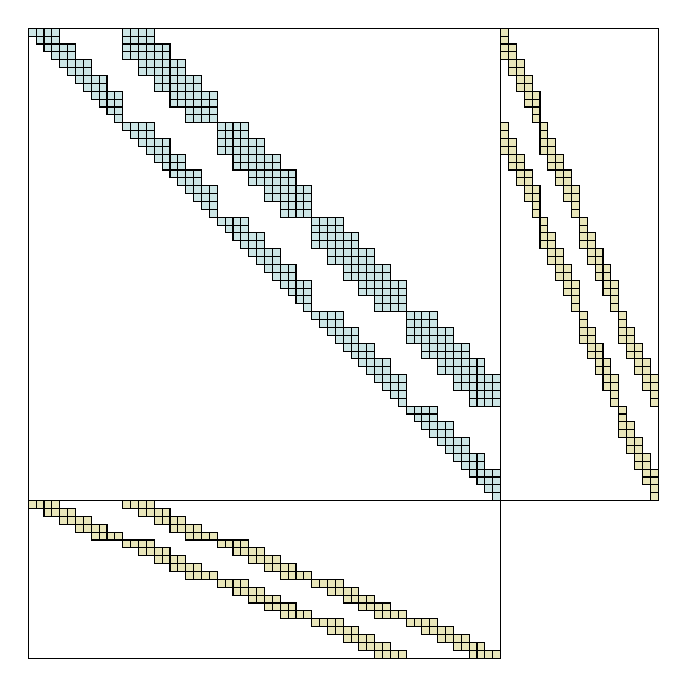
\begin{tikzpicture}
\draw[] (   0.1,   2.1) rectangle (   6.1,   8.1);
\draw[fill=teal!20] (   0.1,   8.0) rectangle (   0.2,   8.1);
\draw[fill=teal!20] (   0.2,   8.0) rectangle (   0.3,   8.1);
\draw[fill=teal!20] (   0.3,   8.0) rectangle (   0.4,   8.1);
\draw[fill=teal!20] (   0.4,   8.0) rectangle (   0.5,   8.1);
\draw[fill=teal!20] (   1.3,   8.0) rectangle (   1.4,   8.1);
\draw[fill=teal!20] (   1.4,   8.0) rectangle (   1.5,   8.1);
\draw[fill=teal!20] (   1.5,   8.0) rectangle (   1.6,   8.1);
\draw[fill=teal!20] (   1.6,   8.0) rectangle (   1.7,   8.1);
\draw[fill=teal!20] (   0.2,   7.9) rectangle (   0.3,   8.0);
\draw[fill=teal!20] (   0.3,   7.9) rectangle (   0.4,   8.0);
\draw[fill=teal!20] (   0.4,   7.9) rectangle (   0.5,   8.0);
\draw[fill=teal!20] (   1.3,   7.9) rectangle (   1.4,   8.0);
\draw[fill=teal!20] (   1.4,   7.9) rectangle (   1.5,   8.0);
\draw[fill=teal!20] (   1.5,   7.9) rectangle (   1.6,   8.0);
\draw[fill=teal!20] (   1.6,   7.9) rectangle (   1.7,   8.0);
\draw[fill=teal!20] (   0.3,   7.8) rectangle (   0.4,   7.9);
\draw[fill=teal!20] (   0.4,   7.8) rectangle (   0.5,   7.9);
\draw[fill=teal!20] (   0.5,   7.8) rectangle (   0.6,   7.9);
\draw[fill=teal!20] (   0.6,   7.8) rectangle (   0.7,   7.9);
\draw[fill=teal!20] (   1.3,   7.8) rectangle (   1.4,   7.9);
\draw[fill=teal!20] (   1.4,   7.8) rectangle (   1.5,   7.9);
\draw[fill=teal!20] (   1.5,   7.8) rectangle (   1.6,   7.9);
\draw[fill=teal!20] (   1.6,   7.8) rectangle (   1.7,   7.9);
\draw[fill=teal!20] (   1.7,   7.8) rectangle (   1.8,   7.9);
\draw[fill=teal!20] (   1.8,   7.8) rectangle (   1.9,   7.9);
\draw[fill=teal!20] (   0.4,   7.7) rectangle (   0.5,   7.8);
\draw[fill=teal!20] (   0.5,   7.7) rectangle (   0.6,   7.8);
\draw[fill=teal!20] (   0.6,   7.7) rectangle (   0.7,   7.8);
\draw[fill=teal!20] (   1.3,   7.7) rectangle (   1.4,   7.8);
\draw[fill=teal!20] (   1.4,   7.7) rectangle (   1.5,   7.8);
\draw[fill=teal!20] (   1.5,   7.7) rectangle (   1.6,   7.8);
\draw[fill=teal!20] (   1.6,   7.7) rectangle (   1.7,   7.8);
\draw[fill=teal!20] (   1.7,   7.7) rectangle (   1.8,   7.8);
\draw[fill=teal!20] (   1.8,   7.7) rectangle (   1.9,   7.8);
\draw[fill=teal!20] (   0.5,   7.6) rectangle (   0.6,   7.7);
\draw[fill=teal!20] (   0.6,   7.6) rectangle (   0.7,   7.7);
\draw[fill=teal!20] (   0.7,   7.6) rectangle (   0.8,   7.7);
\draw[fill=teal!20] (   0.8,   7.6) rectangle (   0.9,   7.7);
\draw[fill=teal!20] (   1.5,   7.6) rectangle (   1.6,   7.7);
\draw[fill=teal!20] (   1.6,   7.6) rectangle (   1.7,   7.7);
\draw[fill=teal!20] (   1.7,   7.6) rectangle (   1.8,   7.7);
\draw[fill=teal!20] (   1.8,   7.6) rectangle (   1.9,   7.7);
\draw[fill=teal!20] (   1.9,   7.6) rectangle (   2.0,   7.7);
\draw[fill=teal!20] (   2.0,   7.6) rectangle (   2.1,   7.7);
\draw[fill=teal!20] (   0.6,   7.5) rectangle (   0.7,   7.6);
\draw[fill=teal!20] (   0.7,   7.5) rectangle (   0.8,   7.6);
\draw[fill=teal!20] (   0.8,   7.5) rectangle (   0.9,   7.6);
\draw[fill=teal!20] (   1.5,   7.5) rectangle (   1.6,   7.6);
\draw[fill=teal!20] (   1.6,   7.5) rectangle (   1.7,   7.6);
\draw[fill=teal!20] (   1.7,   7.5) rectangle (   1.8,   7.6);
\draw[fill=teal!20] (   1.8,   7.5) rectangle (   1.9,   7.6);
\draw[fill=teal!20] (   1.9,   7.5) rectangle (   2.0,   7.6);
\draw[fill=teal!20] (   2.0,   7.5) rectangle (   2.1,   7.6);
\draw[fill=teal!20] (   0.7,   7.4) rectangle (   0.8,   7.5);
\draw[fill=teal!20] (   0.8,   7.4) rectangle (   0.9,   7.5);
\draw[fill=teal!20] (   0.9,   7.4) rectangle (   1.0,   7.5);
\draw[fill=teal!20] (   1.0,   7.4) rectangle (   1.1,   7.5);
\draw[fill=teal!20] (   1.7,   7.4) rectangle (   1.8,   7.5);
\draw[fill=teal!20] (   1.8,   7.4) rectangle (   1.9,   7.5);
\draw[fill=teal!20] (   1.9,   7.4) rectangle (   2.0,   7.5);
\draw[fill=teal!20] (   2.0,   7.4) rectangle (   2.1,   7.5);
\draw[fill=teal!20] (   2.1,   7.4) rectangle (   2.2,   7.5);
\draw[fill=teal!20] (   2.2,   7.4) rectangle (   2.3,   7.5);
\draw[fill=teal!20] (   0.8,   7.3) rectangle (   0.9,   7.4);
\draw[fill=teal!20] (   0.9,   7.3) rectangle (   1.0,   7.4);
\draw[fill=teal!20] (   1.0,   7.3) rectangle (   1.1,   7.4);
\draw[fill=teal!20] (   1.7,   7.3) rectangle (   1.8,   7.4);
\draw[fill=teal!20] (   1.8,   7.3) rectangle (   1.9,   7.4);
\draw[fill=teal!20] (   1.9,   7.3) rectangle (   2.0,   7.4);
\draw[fill=teal!20] (   2.0,   7.3) rectangle (   2.1,   7.4);
\draw[fill=teal!20] (   2.1,   7.3) rectangle (   2.2,   7.4);
\draw[fill=teal!20] (   2.2,   7.3) rectangle (   2.3,   7.4);
\draw[fill=teal!20] (   0.9,   7.2) rectangle (   1.0,   7.3);
\draw[fill=teal!20] (   1.0,   7.2) rectangle (   1.1,   7.3);
\draw[fill=teal!20] (   1.1,   7.2) rectangle (   1.2,   7.3);
\draw[fill=teal!20] (   1.2,   7.2) rectangle (   1.3,   7.3);
\draw[fill=teal!20] (   1.9,   7.2) rectangle (   2.0,   7.3);
\draw[fill=teal!20] (   2.0,   7.2) rectangle (   2.1,   7.3);
\draw[fill=teal!20] (   2.1,   7.2) rectangle (   2.2,   7.3);
\draw[fill=teal!20] (   2.2,   7.2) rectangle (   2.3,   7.3);
\draw[fill=teal!20] (   2.3,   7.2) rectangle (   2.4,   7.3);
\draw[fill=teal!20] (   2.4,   7.2) rectangle (   2.5,   7.3);
\draw[fill=teal!20] (   1.0,   7.1) rectangle (   1.1,   7.2);
\draw[fill=teal!20] (   1.1,   7.1) rectangle (   1.2,   7.2);
\draw[fill=teal!20] (   1.2,   7.1) rectangle (   1.3,   7.2);
\draw[fill=teal!20] (   1.9,   7.1) rectangle (   2.0,   7.2);
\draw[fill=teal!20] (   2.0,   7.1) rectangle (   2.1,   7.2);
\draw[fill=teal!20] (   2.1,   7.1) rectangle (   2.2,   7.2);
\draw[fill=teal!20] (   2.2,   7.1) rectangle (   2.3,   7.2);
\draw[fill=teal!20] (   2.3,   7.1) rectangle (   2.4,   7.2);
\draw[fill=teal!20] (   2.4,   7.1) rectangle (   2.5,   7.2);
\draw[fill=teal!20] (   1.1,   7.0) rectangle (   1.2,   7.1);
\draw[fill=teal!20] (   1.2,   7.0) rectangle (   1.3,   7.1);
\draw[fill=teal!20] (   2.1,   7.0) rectangle (   2.2,   7.1);
\draw[fill=teal!20] (   2.2,   7.0) rectangle (   2.3,   7.1);
\draw[fill=teal!20] (   2.3,   7.0) rectangle (   2.4,   7.1);
\draw[fill=teal!20] (   2.4,   7.0) rectangle (   2.5,   7.1);
\draw[fill=teal!20] (   1.2,   6.9) rectangle (   1.3,   7.0);
\draw[fill=teal!20] (   2.1,   6.9) rectangle (   2.2,   7.0);
\draw[fill=teal!20] (   2.2,   6.9) rectangle (   2.3,   7.0);
\draw[fill=teal!20] (   2.3,   6.9) rectangle (   2.4,   7.0);
\draw[fill=teal!20] (   2.4,   6.9) rectangle (   2.5,   7.0);
\draw[fill=teal!20] (   1.3,   6.8) rectangle (   1.4,   6.9);
\draw[fill=teal!20] (   1.4,   6.8) rectangle (   1.5,   6.9);
\draw[fill=teal!20] (   1.5,   6.8) rectangle (   1.6,   6.9);
\draw[fill=teal!20] (   1.6,   6.8) rectangle (   1.7,   6.9);
\draw[fill=teal!20] (   2.5,   6.8) rectangle (   2.6,   6.9);
\draw[fill=teal!20] (   2.6,   6.8) rectangle (   2.7,   6.9);
\draw[fill=teal!20] (   2.7,   6.8) rectangle (   2.8,   6.9);
\draw[fill=teal!20] (   2.8,   6.8) rectangle (   2.9,   6.9);
\draw[fill=teal!20] (   1.4,   6.7) rectangle (   1.5,   6.8);
\draw[fill=teal!20] (   1.5,   6.7) rectangle (   1.6,   6.8);
\draw[fill=teal!20] (   1.6,   6.7) rectangle (   1.7,   6.8);
\draw[fill=teal!20] (   2.5,   6.7) rectangle (   2.6,   6.8);
\draw[fill=teal!20] (   2.6,   6.7) rectangle (   2.7,   6.8);
\draw[fill=teal!20] (   2.7,   6.7) rectangle (   2.8,   6.8);
\draw[fill=teal!20] (   2.8,   6.7) rectangle (   2.9,   6.8);
\draw[fill=teal!20] (   1.5,   6.6) rectangle (   1.6,   6.7);
\draw[fill=teal!20] (   1.6,   6.6) rectangle (   1.7,   6.7);
\draw[fill=teal!20] (   1.7,   6.6) rectangle (   1.8,   6.7);
\draw[fill=teal!20] (   1.8,   6.6) rectangle (   1.9,   6.7);
\draw[fill=teal!20] (   2.5,   6.6) rectangle (   2.6,   6.7);
\draw[fill=teal!20] (   2.6,   6.6) rectangle (   2.7,   6.7);
\draw[fill=teal!20] (   2.7,   6.6) rectangle (   2.8,   6.7);
\draw[fill=teal!20] (   2.8,   6.6) rectangle (   2.9,   6.7);
\draw[fill=teal!20] (   2.9,   6.6) rectangle (   3.0,   6.7);
\draw[fill=teal!20] (   3.0,   6.6) rectangle (   3.1,   6.7);
\draw[fill=teal!20] (   1.6,   6.5) rectangle (   1.7,   6.6);
\draw[fill=teal!20] (   1.7,   6.5) rectangle (   1.8,   6.6);
\draw[fill=teal!20] (   1.8,   6.5) rectangle (   1.9,   6.6);
\draw[fill=teal!20] (   2.5,   6.5) rectangle (   2.6,   6.6);
\draw[fill=teal!20] (   2.6,   6.5) rectangle (   2.7,   6.6);
\draw[fill=teal!20] (   2.7,   6.5) rectangle (   2.8,   6.6);
\draw[fill=teal!20] (   2.8,   6.5) rectangle (   2.9,   6.6);
\draw[fill=teal!20] (   2.9,   6.5) rectangle (   3.0,   6.6);
\draw[fill=teal!20] (   3.0,   6.5) rectangle (   3.1,   6.6);
\draw[fill=teal!20] (   1.7,   6.4) rectangle (   1.8,   6.5);
\draw[fill=teal!20] (   1.8,   6.4) rectangle (   1.9,   6.5);
\draw[fill=teal!20] (   1.9,   6.4) rectangle (   2.0,   6.5);
\draw[fill=teal!20] (   2.0,   6.4) rectangle (   2.1,   6.5);
\draw[fill=teal!20] (   2.7,   6.4) rectangle (   2.8,   6.5);
\draw[fill=teal!20] (   2.8,   6.4) rectangle (   2.9,   6.5);
\draw[fill=teal!20] (   2.9,   6.4) rectangle (   3.0,   6.5);
\draw[fill=teal!20] (   3.0,   6.4) rectangle (   3.1,   6.5);
\draw[fill=teal!20] (   3.1,   6.4) rectangle (   3.2,   6.5);
\draw[fill=teal!20] (   3.2,   6.4) rectangle (   3.3,   6.5);
\draw[fill=teal!20] (   1.8,   6.3) rectangle (   1.9,   6.4);
\draw[fill=teal!20] (   1.9,   6.3) rectangle (   2.0,   6.4);
\draw[fill=teal!20] (   2.0,   6.3) rectangle (   2.1,   6.4);
\draw[fill=teal!20] (   2.7,   6.3) rectangle (   2.8,   6.4);
\draw[fill=teal!20] (   2.8,   6.3) rectangle (   2.9,   6.4);
\draw[fill=teal!20] (   2.9,   6.3) rectangle (   3.0,   6.4);
\draw[fill=teal!20] (   3.0,   6.3) rectangle (   3.1,   6.4);
\draw[fill=teal!20] (   3.1,   6.3) rectangle (   3.2,   6.4);
\draw[fill=teal!20] (   3.2,   6.3) rectangle (   3.3,   6.4);
\draw[fill=teal!20] (   1.9,   6.2) rectangle (   2.0,   6.3);
\draw[fill=teal!20] (   2.0,   6.2) rectangle (   2.1,   6.3);
\draw[fill=teal!20] (   2.1,   6.2) rectangle (   2.2,   6.3);
\draw[fill=teal!20] (   2.2,   6.2) rectangle (   2.3,   6.3);
\draw[fill=teal!20] (   2.9,   6.2) rectangle (   3.0,   6.3);
\draw[fill=teal!20] (   3.0,   6.2) rectangle (   3.1,   6.3);
\draw[fill=teal!20] (   3.1,   6.2) rectangle (   3.2,   6.3);
\draw[fill=teal!20] (   3.2,   6.2) rectangle (   3.3,   6.3);
\draw[fill=teal!20] (   3.3,   6.2) rectangle (   3.4,   6.3);
\draw[fill=teal!20] (   3.4,   6.2) rectangle (   3.5,   6.3);
\draw[fill=teal!20] (   2.0,   6.1) rectangle (   2.1,   6.2);
\draw[fill=teal!20] (   2.1,   6.1) rectangle (   2.2,   6.2);
\draw[fill=teal!20] (   2.2,   6.1) rectangle (   2.3,   6.2);
\draw[fill=teal!20] (   2.9,   6.1) rectangle (   3.0,   6.2);
\draw[fill=teal!20] (   3.0,   6.1) rectangle (   3.1,   6.2);
\draw[fill=teal!20] (   3.1,   6.1) rectangle (   3.2,   6.2);
\draw[fill=teal!20] (   3.2,   6.1) rectangle (   3.3,   6.2);
\draw[fill=teal!20] (   3.3,   6.1) rectangle (   3.4,   6.2);
\draw[fill=teal!20] (   3.4,   6.1) rectangle (   3.5,   6.2);
\draw[fill=teal!20] (   2.1,   6.0) rectangle (   2.2,   6.1);
\draw[fill=teal!20] (   2.2,   6.0) rectangle (   2.3,   6.1);
\draw[fill=teal!20] (   2.3,   6.0) rectangle (   2.4,   6.1);
\draw[fill=teal!20] (   2.4,   6.0) rectangle (   2.5,   6.1);
\draw[fill=teal!20] (   3.1,   6.0) rectangle (   3.2,   6.1);
\draw[fill=teal!20] (   3.2,   6.0) rectangle (   3.3,   6.1);
\draw[fill=teal!20] (   3.3,   6.0) rectangle (   3.4,   6.1);
\draw[fill=teal!20] (   3.4,   6.0) rectangle (   3.5,   6.1);
\draw[fill=teal!20] (   3.5,   6.0) rectangle (   3.6,   6.1);
\draw[fill=teal!20] (   3.6,   6.0) rectangle (   3.7,   6.1);
\draw[fill=teal!20] (   2.2,   5.9) rectangle (   2.3,   6.0);
\draw[fill=teal!20] (   2.3,   5.9) rectangle (   2.4,   6.0);
\draw[fill=teal!20] (   2.4,   5.9) rectangle (   2.5,   6.0);
\draw[fill=teal!20] (   3.1,   5.9) rectangle (   3.2,   6.0);
\draw[fill=teal!20] (   3.2,   5.9) rectangle (   3.3,   6.0);
\draw[fill=teal!20] (   3.3,   5.9) rectangle (   3.4,   6.0);
\draw[fill=teal!20] (   3.4,   5.9) rectangle (   3.5,   6.0);
\draw[fill=teal!20] (   3.5,   5.9) rectangle (   3.6,   6.0);
\draw[fill=teal!20] (   3.6,   5.9) rectangle (   3.7,   6.0);
\draw[fill=teal!20] (   2.3,   5.8) rectangle (   2.4,   5.9);
\draw[fill=teal!20] (   2.4,   5.8) rectangle (   2.5,   5.9);
\draw[fill=teal!20] (   3.3,   5.8) rectangle (   3.4,   5.9);
\draw[fill=teal!20] (   3.4,   5.8) rectangle (   3.5,   5.9);
\draw[fill=teal!20] (   3.5,   5.8) rectangle (   3.6,   5.9);
\draw[fill=teal!20] (   3.6,   5.8) rectangle (   3.7,   5.9);
\draw[fill=teal!20] (   2.4,   5.7) rectangle (   2.5,   5.8);
\draw[fill=teal!20] (   3.3,   5.7) rectangle (   3.4,   5.8);
\draw[fill=teal!20] (   3.4,   5.7) rectangle (   3.5,   5.8);
\draw[fill=teal!20] (   3.5,   5.7) rectangle (   3.6,   5.8);
\draw[fill=teal!20] (   3.6,   5.7) rectangle (   3.7,   5.8);
\draw[fill=teal!20] (   2.5,   5.6) rectangle (   2.6,   5.7);
\draw[fill=teal!20] (   2.6,   5.6) rectangle (   2.7,   5.7);
\draw[fill=teal!20] (   2.7,   5.6) rectangle (   2.8,   5.7);
\draw[fill=teal!20] (   2.8,   5.6) rectangle (   2.9,   5.7);
\draw[fill=teal!20] (   3.7,   5.6) rectangle (   3.8,   5.7);
\draw[fill=teal!20] (   3.8,   5.6) rectangle (   3.9,   5.7);
\draw[fill=teal!20] (   3.9,   5.6) rectangle (   4.0,   5.7);
\draw[fill=teal!20] (   4.0,   5.6) rectangle (   4.1,   5.7);
\draw[fill=teal!20] (   2.6,   5.5) rectangle (   2.7,   5.6);
\draw[fill=teal!20] (   2.7,   5.5) rectangle (   2.8,   5.6);
\draw[fill=teal!20] (   2.8,   5.5) rectangle (   2.9,   5.6);
\draw[fill=teal!20] (   3.7,   5.5) rectangle (   3.8,   5.6);
\draw[fill=teal!20] (   3.8,   5.5) rectangle (   3.9,   5.6);
\draw[fill=teal!20] (   3.9,   5.5) rectangle (   4.0,   5.6);
\draw[fill=teal!20] (   4.0,   5.5) rectangle (   4.1,   5.6);
\draw[fill=teal!20] (   2.7,   5.4) rectangle (   2.8,   5.5);
\draw[fill=teal!20] (   2.8,   5.4) rectangle (   2.9,   5.5);
\draw[fill=teal!20] (   2.9,   5.4) rectangle (   3.0,   5.5);
\draw[fill=teal!20] (   3.0,   5.4) rectangle (   3.1,   5.5);
\draw[fill=teal!20] (   3.7,   5.4) rectangle (   3.8,   5.5);
\draw[fill=teal!20] (   3.8,   5.4) rectangle (   3.9,   5.5);
\draw[fill=teal!20] (   3.9,   5.4) rectangle (   4.0,   5.5);
\draw[fill=teal!20] (   4.0,   5.4) rectangle (   4.1,   5.5);
\draw[fill=teal!20] (   4.1,   5.4) rectangle (   4.2,   5.5);
\draw[fill=teal!20] (   4.2,   5.4) rectangle (   4.3,   5.5);
\draw[fill=teal!20] (   2.8,   5.3) rectangle (   2.9,   5.4);
\draw[fill=teal!20] (   2.9,   5.3) rectangle (   3.0,   5.4);
\draw[fill=teal!20] (   3.0,   5.3) rectangle (   3.1,   5.4);
\draw[fill=teal!20] (   3.7,   5.3) rectangle (   3.8,   5.4);
\draw[fill=teal!20] (   3.8,   5.3) rectangle (   3.9,   5.4);
\draw[fill=teal!20] (   3.9,   5.3) rectangle (   4.0,   5.4);
\draw[fill=teal!20] (   4.0,   5.3) rectangle (   4.1,   5.4);
\draw[fill=teal!20] (   4.1,   5.3) rectangle (   4.2,   5.4);
\draw[fill=teal!20] (   4.2,   5.3) rectangle (   4.3,   5.4);
\draw[fill=teal!20] (   2.9,   5.2) rectangle (   3.0,   5.3);
\draw[fill=teal!20] (   3.0,   5.2) rectangle (   3.1,   5.3);
\draw[fill=teal!20] (   3.1,   5.2) rectangle (   3.2,   5.3);
\draw[fill=teal!20] (   3.2,   5.2) rectangle (   3.3,   5.3);
\draw[fill=teal!20] (   3.9,   5.2) rectangle (   4.0,   5.3);
\draw[fill=teal!20] (   4.0,   5.2) rectangle (   4.1,   5.3);
\draw[fill=teal!20] (   4.1,   5.2) rectangle (   4.2,   5.3);
\draw[fill=teal!20] (   4.2,   5.2) rectangle (   4.3,   5.3);
\draw[fill=teal!20] (   4.3,   5.2) rectangle (   4.4,   5.3);
\draw[fill=teal!20] (   4.4,   5.2) rectangle (   4.5,   5.3);
\draw[fill=teal!20] (   3.0,   5.1) rectangle (   3.1,   5.2);
\draw[fill=teal!20] (   3.1,   5.1) rectangle (   3.2,   5.2);
\draw[fill=teal!20] (   3.2,   5.1) rectangle (   3.3,   5.2);
\draw[fill=teal!20] (   3.9,   5.1) rectangle (   4.0,   5.2);
\draw[fill=teal!20] (   4.0,   5.1) rectangle (   4.1,   5.2);
\draw[fill=teal!20] (   4.1,   5.1) rectangle (   4.2,   5.2);
\draw[fill=teal!20] (   4.2,   5.1) rectangle (   4.3,   5.2);
\draw[fill=teal!20] (   4.3,   5.1) rectangle (   4.4,   5.2);
\draw[fill=teal!20] (   4.4,   5.1) rectangle (   4.5,   5.2);
\draw[fill=teal!20] (   3.1,   5.0) rectangle (   3.2,   5.1);
\draw[fill=teal!20] (   3.2,   5.0) rectangle (   3.3,   5.1);
\draw[fill=teal!20] (   3.3,   5.0) rectangle (   3.4,   5.1);
\draw[fill=teal!20] (   3.4,   5.0) rectangle (   3.5,   5.1);
\draw[fill=teal!20] (   4.1,   5.0) rectangle (   4.2,   5.1);
\draw[fill=teal!20] (   4.2,   5.0) rectangle (   4.3,   5.1);
\draw[fill=teal!20] (   4.3,   5.0) rectangle (   4.4,   5.1);
\draw[fill=teal!20] (   4.4,   5.0) rectangle (   4.5,   5.1);
\draw[fill=teal!20] (   4.5,   5.0) rectangle (   4.6,   5.1);
\draw[fill=teal!20] (   4.6,   5.0) rectangle (   4.7,   5.1);
\draw[fill=teal!20] (   3.2,   4.9) rectangle (   3.3,   5.0);
\draw[fill=teal!20] (   3.3,   4.9) rectangle (   3.4,   5.0);
\draw[fill=teal!20] (   3.4,   4.9) rectangle (   3.5,   5.0);
\draw[fill=teal!20] (   4.1,   4.9) rectangle (   4.2,   5.0);
\draw[fill=teal!20] (   4.2,   4.9) rectangle (   4.3,   5.0);
\draw[fill=teal!20] (   4.3,   4.9) rectangle (   4.4,   5.0);
\draw[fill=teal!20] (   4.4,   4.9) rectangle (   4.5,   5.0);
\draw[fill=teal!20] (   4.5,   4.9) rectangle (   4.6,   5.0);
\draw[fill=teal!20] (   4.6,   4.9) rectangle (   4.7,   5.0);
\draw[fill=teal!20] (   3.3,   4.8) rectangle (   3.4,   4.9);
\draw[fill=teal!20] (   3.4,   4.8) rectangle (   3.5,   4.9);
\draw[fill=teal!20] (   3.5,   4.8) rectangle (   3.6,   4.9);
\draw[fill=teal!20] (   3.6,   4.8) rectangle (   3.7,   4.9);
\draw[fill=teal!20] (   4.3,   4.8) rectangle (   4.4,   4.9);
\draw[fill=teal!20] (   4.4,   4.8) rectangle (   4.5,   4.9);
\draw[fill=teal!20] (   4.5,   4.8) rectangle (   4.6,   4.9);
\draw[fill=teal!20] (   4.6,   4.8) rectangle (   4.7,   4.9);
\draw[fill=teal!20] (   4.7,   4.8) rectangle (   4.8,   4.9);
\draw[fill=teal!20] (   4.8,   4.8) rectangle (   4.9,   4.9);
\draw[fill=teal!20] (   3.4,   4.7) rectangle (   3.5,   4.8);
\draw[fill=teal!20] (   3.5,   4.7) rectangle (   3.6,   4.8);
\draw[fill=teal!20] (   3.6,   4.7) rectangle (   3.7,   4.8);
\draw[fill=teal!20] (   4.3,   4.7) rectangle (   4.4,   4.8);
\draw[fill=teal!20] (   4.4,   4.7) rectangle (   4.5,   4.8);
\draw[fill=teal!20] (   4.5,   4.7) rectangle (   4.6,   4.8);
\draw[fill=teal!20] (   4.6,   4.7) rectangle (   4.7,   4.8);
\draw[fill=teal!20] (   4.7,   4.7) rectangle (   4.8,   4.8);
\draw[fill=teal!20] (   4.8,   4.7) rectangle (   4.9,   4.8);
\draw[fill=teal!20] (   3.5,   4.6) rectangle (   3.6,   4.7);
\draw[fill=teal!20] (   3.6,   4.6) rectangle (   3.7,   4.7);
\draw[fill=teal!20] (   4.5,   4.6) rectangle (   4.6,   4.7);
\draw[fill=teal!20] (   4.6,   4.6) rectangle (   4.7,   4.7);
\draw[fill=teal!20] (   4.7,   4.6) rectangle (   4.8,   4.7);
\draw[fill=teal!20] (   4.8,   4.6) rectangle (   4.9,   4.7);
\draw[fill=teal!20] (   3.6,   4.5) rectangle (   3.7,   4.6);
\draw[fill=teal!20] (   4.5,   4.5) rectangle (   4.6,   4.6);
\draw[fill=teal!20] (   4.6,   4.5) rectangle (   4.7,   4.6);
\draw[fill=teal!20] (   4.7,   4.5) rectangle (   4.8,   4.6);
\draw[fill=teal!20] (   4.8,   4.5) rectangle (   4.9,   4.6);
\draw[fill=teal!20] (   3.7,   4.4) rectangle (   3.8,   4.5);
\draw[fill=teal!20] (   3.8,   4.4) rectangle (   3.9,   4.5);
\draw[fill=teal!20] (   3.9,   4.4) rectangle (   4.0,   4.5);
\draw[fill=teal!20] (   4.0,   4.4) rectangle (   4.1,   4.5);
\draw[fill=teal!20] (   4.9,   4.4) rectangle (   5.0,   4.5);
\draw[fill=teal!20] (   5.0,   4.4) rectangle (   5.1,   4.5);
\draw[fill=teal!20] (   5.1,   4.4) rectangle (   5.2,   4.5);
\draw[fill=teal!20] (   5.2,   4.4) rectangle (   5.3,   4.5);
\draw[fill=teal!20] (   3.8,   4.3) rectangle (   3.9,   4.4);
\draw[fill=teal!20] (   3.9,   4.3) rectangle (   4.0,   4.4);
\draw[fill=teal!20] (   4.0,   4.3) rectangle (   4.1,   4.4);
\draw[fill=teal!20] (   4.9,   4.3) rectangle (   5.0,   4.4);
\draw[fill=teal!20] (   5.0,   4.3) rectangle (   5.1,   4.4);
\draw[fill=teal!20] (   5.1,   4.3) rectangle (   5.2,   4.4);
\draw[fill=teal!20] (   5.2,   4.3) rectangle (   5.3,   4.4);
\draw[fill=teal!20] (   3.9,   4.2) rectangle (   4.0,   4.3);
\draw[fill=teal!20] (   4.0,   4.2) rectangle (   4.1,   4.3);
\draw[fill=teal!20] (   4.1,   4.2) rectangle (   4.2,   4.3);
\draw[fill=teal!20] (   4.2,   4.2) rectangle (   4.3,   4.3);
\draw[fill=teal!20] (   4.9,   4.2) rectangle (   5.0,   4.3);
\draw[fill=teal!20] (   5.0,   4.2) rectangle (   5.1,   4.3);
\draw[fill=teal!20] (   5.1,   4.2) rectangle (   5.2,   4.3);
\draw[fill=teal!20] (   5.2,   4.2) rectangle (   5.3,   4.3);
\draw[fill=teal!20] (   5.3,   4.2) rectangle (   5.4,   4.3);
\draw[fill=teal!20] (   5.4,   4.2) rectangle (   5.5,   4.3);
\draw[fill=teal!20] (   4.0,   4.1) rectangle (   4.1,   4.2);
\draw[fill=teal!20] (   4.1,   4.1) rectangle (   4.2,   4.2);
\draw[fill=teal!20] (   4.2,   4.1) rectangle (   4.3,   4.2);
\draw[fill=teal!20] (   4.9,   4.1) rectangle (   5.0,   4.2);
\draw[fill=teal!20] (   5.0,   4.1) rectangle (   5.1,   4.2);
\draw[fill=teal!20] (   5.1,   4.1) rectangle (   5.2,   4.2);
\draw[fill=teal!20] (   5.2,   4.1) rectangle (   5.3,   4.2);
\draw[fill=teal!20] (   5.3,   4.1) rectangle (   5.4,   4.2);
\draw[fill=teal!20] (   5.4,   4.1) rectangle (   5.5,   4.2);
\draw[fill=teal!20] (   4.1,   4.0) rectangle (   4.2,   4.1);
\draw[fill=teal!20] (   4.2,   4.0) rectangle (   4.3,   4.1);
\draw[fill=teal!20] (   4.3,   4.0) rectangle (   4.4,   4.1);
\draw[fill=teal!20] (   4.4,   4.0) rectangle (   4.5,   4.1);
\draw[fill=teal!20] (   5.1,   4.0) rectangle (   5.2,   4.1);
\draw[fill=teal!20] (   5.2,   4.0) rectangle (   5.3,   4.1);
\draw[fill=teal!20] (   5.3,   4.0) rectangle (   5.4,   4.1);
\draw[fill=teal!20] (   5.4,   4.0) rectangle (   5.5,   4.1);
\draw[fill=teal!20] (   5.5,   4.0) rectangle (   5.6,   4.1);
\draw[fill=teal!20] (   5.6,   4.0) rectangle (   5.7,   4.1);
\draw[fill=teal!20] (   4.2,   3.9) rectangle (   4.3,   4.0);
\draw[fill=teal!20] (   4.3,   3.9) rectangle (   4.4,   4.0);
\draw[fill=teal!20] (   4.4,   3.9) rectangle (   4.5,   4.0);
\draw[fill=teal!20] (   5.1,   3.9) rectangle (   5.2,   4.0);
\draw[fill=teal!20] (   5.2,   3.9) rectangle (   5.3,   4.0);
\draw[fill=teal!20] (   5.3,   3.9) rectangle (   5.4,   4.0);
\draw[fill=teal!20] (   5.4,   3.9) rectangle (   5.5,   4.0);
\draw[fill=teal!20] (   5.5,   3.9) rectangle (   5.6,   4.0);
\draw[fill=teal!20] (   5.6,   3.9) rectangle (   5.7,   4.0);
\draw[fill=teal!20] (   4.3,   3.8) rectangle (   4.4,   3.9);
\draw[fill=teal!20] (   4.4,   3.8) rectangle (   4.5,   3.9);
\draw[fill=teal!20] (   4.5,   3.8) rectangle (   4.6,   3.9);
\draw[fill=teal!20] (   4.6,   3.8) rectangle (   4.7,   3.9);
\draw[fill=teal!20] (   5.3,   3.8) rectangle (   5.4,   3.9);
\draw[fill=teal!20] (   5.4,   3.8) rectangle (   5.5,   3.9);
\draw[fill=teal!20] (   5.5,   3.8) rectangle (   5.6,   3.9);
\draw[fill=teal!20] (   5.6,   3.8) rectangle (   5.7,   3.9);
\draw[fill=teal!20] (   5.7,   3.8) rectangle (   5.8,   3.9);
\draw[fill=teal!20] (   5.8,   3.8) rectangle (   5.9,   3.9);
\draw[fill=teal!20] (   4.4,   3.7) rectangle (   4.5,   3.8);
\draw[fill=teal!20] (   4.5,   3.7) rectangle (   4.6,   3.8);
\draw[fill=teal!20] (   4.6,   3.7) rectangle (   4.7,   3.8);
\draw[fill=teal!20] (   5.3,   3.7) rectangle (   5.4,   3.8);
\draw[fill=teal!20] (   5.4,   3.7) rectangle (   5.5,   3.8);
\draw[fill=teal!20] (   5.5,   3.7) rectangle (   5.6,   3.8);
\draw[fill=teal!20] (   5.6,   3.7) rectangle (   5.7,   3.8);
\draw[fill=teal!20] (   5.7,   3.7) rectangle (   5.8,   3.8);
\draw[fill=teal!20] (   5.8,   3.7) rectangle (   5.9,   3.8);
\draw[fill=teal!20] (   4.5,   3.6) rectangle (   4.6,   3.7);
\draw[fill=teal!20] (   4.6,   3.6) rectangle (   4.7,   3.7);
\draw[fill=teal!20] (   4.7,   3.6) rectangle (   4.8,   3.7);
\draw[fill=teal!20] (   4.8,   3.6) rectangle (   4.9,   3.7);
\draw[fill=teal!20] (   5.5,   3.6) rectangle (   5.6,   3.7);
\draw[fill=teal!20] (   5.6,   3.6) rectangle (   5.7,   3.7);
\draw[fill=teal!20] (   5.7,   3.6) rectangle (   5.8,   3.7);
\draw[fill=teal!20] (   5.8,   3.6) rectangle (   5.9,   3.7);
\draw[fill=teal!20] (   5.9,   3.6) rectangle (   6.0,   3.7);
\draw[fill=teal!20] (   6.0,   3.6) rectangle (   6.1,   3.7);
\draw[fill=teal!20] (   4.6,   3.5) rectangle (   4.7,   3.6);
\draw[fill=teal!20] (   4.7,   3.5) rectangle (   4.8,   3.6);
\draw[fill=teal!20] (   4.8,   3.5) rectangle (   4.9,   3.6);
\draw[fill=teal!20] (   5.5,   3.5) rectangle (   5.6,   3.6);
\draw[fill=teal!20] (   5.6,   3.5) rectangle (   5.7,   3.6);
\draw[fill=teal!20] (   5.7,   3.5) rectangle (   5.8,   3.6);
\draw[fill=teal!20] (   5.8,   3.5) rectangle (   5.9,   3.6);
\draw[fill=teal!20] (   5.9,   3.5) rectangle (   6.0,   3.6);
\draw[fill=teal!20] (   6.0,   3.5) rectangle (   6.1,   3.6);
\draw[fill=teal!20] (   4.7,   3.4) rectangle (   4.8,   3.5);
\draw[fill=teal!20] (   4.8,   3.4) rectangle (   4.9,   3.5);
\draw[fill=teal!20] (   5.7,   3.4) rectangle (   5.8,   3.5);
\draw[fill=teal!20] (   5.8,   3.4) rectangle (   5.9,   3.5);
\draw[fill=teal!20] (   5.9,   3.4) rectangle (   6.0,   3.5);
\draw[fill=teal!20] (   6.0,   3.4) rectangle (   6.1,   3.5);
\draw[fill=teal!20] (   4.8,   3.3) rectangle (   4.9,   3.4);
\draw[fill=teal!20] (   5.7,   3.3) rectangle (   5.8,   3.4);
\draw[fill=teal!20] (   5.8,   3.3) rectangle (   5.9,   3.4);
\draw[fill=teal!20] (   5.9,   3.3) rectangle (   6.0,   3.4);
\draw[fill=teal!20] (   6.0,   3.3) rectangle (   6.1,   3.4);
\draw[fill=teal!20] (   4.9,   3.2) rectangle (   5.0,   3.3);
\draw[fill=teal!20] (   5.0,   3.2) rectangle (   5.1,   3.3);
\draw[fill=teal!20] (   5.1,   3.2) rectangle (   5.2,   3.3);
\draw[fill=teal!20] (   5.2,   3.2) rectangle (   5.3,   3.3);
\draw[fill=teal!20] (   5.0,   3.1) rectangle (   5.1,   3.2);
\draw[fill=teal!20] (   5.1,   3.1) rectangle (   5.2,   3.2);
\draw[fill=teal!20] (   5.2,   3.1) rectangle (   5.3,   3.2);
\draw[fill=teal!20] (   5.1,   3.0) rectangle (   5.2,   3.1);
\draw[fill=teal!20] (   5.2,   3.0) rectangle (   5.3,   3.1);
\draw[fill=teal!20] (   5.3,   3.0) rectangle (   5.4,   3.1);
\draw[fill=teal!20] (   5.4,   3.0) rectangle (   5.5,   3.1);
\draw[fill=teal!20] (   5.2,   2.9) rectangle (   5.3,   3.0);
\draw[fill=teal!20] (   5.3,   2.9) rectangle (   5.4,   3.0);
\draw[fill=teal!20] (   5.4,   2.9) rectangle (   5.5,   3.0);
\draw[fill=teal!20] (   5.3,   2.8) rectangle (   5.4,   2.9);
\draw[fill=teal!20] (   5.4,   2.8) rectangle (   5.5,   2.9);
\draw[fill=teal!20] (   5.5,   2.8) rectangle (   5.6,   2.9);
\draw[fill=teal!20] (   5.6,   2.8) rectangle (   5.7,   2.9);
\draw[fill=teal!20] (   5.4,   2.7) rectangle (   5.5,   2.8);
\draw[fill=teal!20] (   5.5,   2.7) rectangle (   5.6,   2.8);
\draw[fill=teal!20] (   5.6,   2.7) rectangle (   5.7,   2.8);
\draw[fill=teal!20] (   5.5,   2.6) rectangle (   5.6,   2.7);
\draw[fill=teal!20] (   5.6,   2.6) rectangle (   5.7,   2.7);
\draw[fill=teal!20] (   5.7,   2.6) rectangle (   5.8,   2.7);
\draw[fill=teal!20] (   5.8,   2.6) rectangle (   5.9,   2.7);
\draw[fill=teal!20] (   5.6,   2.5) rectangle (   5.7,   2.6);
\draw[fill=teal!20] (   5.7,   2.5) rectangle (   5.8,   2.6);
\draw[fill=teal!20] (   5.8,   2.5) rectangle (   5.9,   2.6);
\draw[fill=teal!20] (   5.7,   2.4) rectangle (   5.8,   2.5);
\draw[fill=teal!20] (   5.8,   2.4) rectangle (   5.9,   2.5);
\draw[fill=teal!20] (   5.9,   2.4) rectangle (   6.0,   2.5);
\draw[fill=teal!20] (   6.0,   2.4) rectangle (   6.1,   2.5);
\draw[fill=teal!20] (   5.8,   2.3) rectangle (   5.9,   2.4);
\draw[fill=teal!20] (   5.9,   2.3) rectangle (   6.0,   2.4);
\draw[fill=teal!20] (   6.0,   2.3) rectangle (   6.1,   2.4);
\draw[fill=teal!20] (   5.9,   2.2) rectangle (   6.0,   2.3);
\draw[fill=teal!20] (   6.0,   2.2) rectangle (   6.1,   2.3);
\draw[fill=teal!20] (   6.0,   2.1) rectangle (   6.1,   2.2);
\draw[] (   6.1,   2.1) rectangle (   8.1,   8.1);
\draw[fill=olive!20] (   8.0,   2.1) rectangle (   8.1,   2.2);
\draw[fill=olive!20] (   8.0,   2.2) rectangle (   8.1,   2.3);
\draw[fill=olive!20] (   8.0,   2.3) rectangle (   8.1,   2.4);
\draw[fill=olive!20] (   8.0,   2.4) rectangle (   8.1,   2.5);
\draw[fill=olive!20] (   8.0,   3.5) rectangle (   8.1,   3.6);
\draw[fill=olive!20] (   8.0,   3.6) rectangle (   8.1,   3.7);
\draw[fill=olive!20] (   8.0,   3.3) rectangle (   8.1,   3.4);
\draw[fill=olive!20] (   8.0,   3.4) rectangle (   8.1,   3.5);
\draw[fill=olive!20] (   7.9,   2.3) rectangle (   8.0,   2.4);
\draw[fill=olive!20] (   7.9,   2.4) rectangle (   8.0,   2.5);
\draw[fill=olive!20] (   7.9,   2.5) rectangle (   8.0,   2.6);
\draw[fill=olive!20] (   7.9,   2.6) rectangle (   8.0,   2.7);
\draw[fill=olive!20] (   7.9,   3.7) rectangle (   8.0,   3.8);
\draw[fill=olive!20] (   7.9,   3.8) rectangle (   8.0,   3.9);
\draw[fill=olive!20] (   7.9,   3.5) rectangle (   8.0,   3.6);
\draw[fill=olive!20] (   7.9,   3.6) rectangle (   8.0,   3.7);
\draw[fill=olive!20] (   7.8,   2.5) rectangle (   7.9,   2.6);
\draw[fill=olive!20] (   7.8,   2.6) rectangle (   7.9,   2.7);
\draw[fill=olive!20] (   7.8,   2.7) rectangle (   7.9,   2.8);
\draw[fill=olive!20] (   7.8,   2.8) rectangle (   7.9,   2.9);
\draw[fill=olive!20] (   7.8,   3.9) rectangle (   7.9,   4.0);
\draw[fill=olive!20] (   7.8,   4.0) rectangle (   7.9,   4.1);
\draw[fill=olive!20] (   7.8,   3.7) rectangle (   7.9,   3.8);
\draw[fill=olive!20] (   7.8,   3.8) rectangle (   7.9,   3.9);
\draw[fill=olive!20] (   7.7,   2.7) rectangle (   7.8,   2.8);
\draw[fill=olive!20] (   7.7,   2.8) rectangle (   7.8,   2.9);
\draw[fill=olive!20] (   7.7,   2.9) rectangle (   7.8,   3.0);
\draw[fill=olive!20] (   7.7,   3.0) rectangle (   7.8,   3.1);
\draw[fill=olive!20] (   7.7,   4.1) rectangle (   7.8,   4.2);
\draw[fill=olive!20] (   7.7,   4.2) rectangle (   7.8,   4.3);
\draw[fill=olive!20] (   7.7,   3.9) rectangle (   7.8,   4.0);
\draw[fill=olive!20] (   7.7,   4.0) rectangle (   7.8,   4.1);
\draw[fill=olive!20] (   7.6,   2.9) rectangle (   7.7,   3.0);
\draw[fill=olive!20] (   7.6,   3.0) rectangle (   7.7,   3.1);
\draw[fill=olive!20] (   7.6,   3.1) rectangle (   7.7,   3.2);
\draw[fill=olive!20] (   7.6,   3.2) rectangle (   7.7,   3.3);
\draw[fill=olive!20] (   7.6,   4.3) rectangle (   7.7,   4.4);
\draw[fill=olive!20] (   7.6,   4.4) rectangle (   7.7,   4.5);
\draw[fill=olive!20] (   7.6,   4.1) rectangle (   7.7,   4.2);
\draw[fill=olive!20] (   7.6,   4.2) rectangle (   7.7,   4.3);
\draw[fill=olive!20] (   7.5,   3.3) rectangle (   7.6,   3.4);
\draw[fill=olive!20] (   7.5,   3.4) rectangle (   7.6,   3.5);
\draw[fill=olive!20] (   7.5,   3.5) rectangle (   7.6,   3.6);
\draw[fill=olive!20] (   7.5,   3.6) rectangle (   7.6,   3.7);
\draw[fill=olive!20] (   7.5,   4.7) rectangle (   7.6,   4.8);
\draw[fill=olive!20] (   7.5,   4.8) rectangle (   7.6,   4.9);
\draw[fill=olive!20] (   7.5,   4.5) rectangle (   7.6,   4.6);
\draw[fill=olive!20] (   7.5,   4.6) rectangle (   7.6,   4.7);
\draw[fill=olive!20] (   7.4,   3.5) rectangle (   7.5,   3.6);
\draw[fill=olive!20] (   7.4,   3.6) rectangle (   7.5,   3.7);
\draw[fill=olive!20] (   7.4,   3.7) rectangle (   7.5,   3.8);
\draw[fill=olive!20] (   7.4,   3.8) rectangle (   7.5,   3.9);
\draw[fill=olive!20] (   7.4,   4.9) rectangle (   7.5,   5.0);
\draw[fill=olive!20] (   7.4,   5.0) rectangle (   7.5,   5.1);
\draw[fill=olive!20] (   7.4,   4.7) rectangle (   7.5,   4.8);
\draw[fill=olive!20] (   7.4,   4.8) rectangle (   7.5,   4.9);
\draw[fill=olive!20] (   7.3,   3.7) rectangle (   7.4,   3.8);
\draw[fill=olive!20] (   7.3,   3.8) rectangle (   7.4,   3.9);
\draw[fill=olive!20] (   7.3,   3.9) rectangle (   7.4,   4.0);
\draw[fill=olive!20] (   7.3,   4.0) rectangle (   7.4,   4.1);
\draw[fill=olive!20] (   7.3,   5.1) rectangle (   7.4,   5.2);
\draw[fill=olive!20] (   7.3,   5.2) rectangle (   7.4,   5.3);
\draw[fill=olive!20] (   7.3,   4.9) rectangle (   7.4,   5.0);
\draw[fill=olive!20] (   7.3,   5.0) rectangle (   7.4,   5.1);
\draw[fill=olive!20] (   7.2,   3.9) rectangle (   7.3,   4.0);
\draw[fill=olive!20] (   7.2,   4.0) rectangle (   7.3,   4.1);
\draw[fill=olive!20] (   7.2,   4.1) rectangle (   7.3,   4.2);
\draw[fill=olive!20] (   7.2,   4.2) rectangle (   7.3,   4.3);
\draw[fill=olive!20] (   7.2,   5.3) rectangle (   7.3,   5.4);
\draw[fill=olive!20] (   7.2,   5.4) rectangle (   7.3,   5.5);
\draw[fill=olive!20] (   7.2,   5.1) rectangle (   7.3,   5.2);
\draw[fill=olive!20] (   7.2,   5.2) rectangle (   7.3,   5.3);
\draw[fill=olive!20] (   7.1,   4.1) rectangle (   7.2,   4.2);
\draw[fill=olive!20] (   7.1,   4.2) rectangle (   7.2,   4.3);
\draw[fill=olive!20] (   7.1,   4.3) rectangle (   7.2,   4.4);
\draw[fill=olive!20] (   7.1,   4.4) rectangle (   7.2,   4.5);
\draw[fill=olive!20] (   7.1,   5.5) rectangle (   7.2,   5.6);
\draw[fill=olive!20] (   7.1,   5.6) rectangle (   7.2,   5.7);
\draw[fill=olive!20] (   7.1,   5.3) rectangle (   7.2,   5.4);
\draw[fill=olive!20] (   7.1,   5.4) rectangle (   7.2,   5.5);
\draw[fill=olive!20] (   7.0,   4.5) rectangle (   7.1,   4.6);
\draw[fill=olive!20] (   7.0,   4.6) rectangle (   7.1,   4.7);
\draw[fill=olive!20] (   7.0,   4.7) rectangle (   7.1,   4.8);
\draw[fill=olive!20] (   7.0,   4.8) rectangle (   7.1,   4.9);
\draw[fill=olive!20] (   7.0,   5.9) rectangle (   7.1,   6.0);
\draw[fill=olive!20] (   7.0,   6.0) rectangle (   7.1,   6.1);
\draw[fill=olive!20] (   7.0,   5.7) rectangle (   7.1,   5.8);
\draw[fill=olive!20] (   7.0,   5.8) rectangle (   7.1,   5.9);
\draw[fill=olive!20] (   6.9,   4.7) rectangle (   7.0,   4.8);
\draw[fill=olive!20] (   6.9,   4.8) rectangle (   7.0,   4.9);
\draw[fill=olive!20] (   6.9,   4.9) rectangle (   7.0,   5.0);
\draw[fill=olive!20] (   6.9,   5.0) rectangle (   7.0,   5.1);
\draw[fill=olive!20] (   6.9,   6.1) rectangle (   7.0,   6.2);
\draw[fill=olive!20] (   6.9,   6.2) rectangle (   7.0,   6.3);
\draw[fill=olive!20] (   6.9,   5.9) rectangle (   7.0,   6.0);
\draw[fill=olive!20] (   6.9,   6.0) rectangle (   7.0,   6.1);
\draw[fill=olive!20] (   6.8,   4.9) rectangle (   6.9,   5.0);
\draw[fill=olive!20] (   6.8,   5.0) rectangle (   6.9,   5.1);
\draw[fill=olive!20] (   6.8,   5.1) rectangle (   6.9,   5.2);
\draw[fill=olive!20] (   6.8,   5.2) rectangle (   6.9,   5.3);
\draw[fill=olive!20] (   6.8,   6.3) rectangle (   6.9,   6.4);
\draw[fill=olive!20] (   6.8,   6.4) rectangle (   6.9,   6.5);
\draw[fill=olive!20] (   6.8,   6.1) rectangle (   6.9,   6.2);
\draw[fill=olive!20] (   6.8,   6.2) rectangle (   6.9,   6.3);
\draw[fill=olive!20] (   6.7,   5.1) rectangle (   6.8,   5.2);
\draw[fill=olive!20] (   6.7,   5.2) rectangle (   6.8,   5.3);
\draw[fill=olive!20] (   6.7,   5.3) rectangle (   6.8,   5.4);
\draw[fill=olive!20] (   6.7,   5.4) rectangle (   6.8,   5.5);
\draw[fill=olive!20] (   6.7,   6.5) rectangle (   6.8,   6.6);
\draw[fill=olive!20] (   6.7,   6.6) rectangle (   6.8,   6.7);
\draw[fill=olive!20] (   6.7,   6.3) rectangle (   6.8,   6.4);
\draw[fill=olive!20] (   6.7,   6.4) rectangle (   6.8,   6.5);
\draw[fill=olive!20] (   6.6,   5.3) rectangle (   6.7,   5.4);
\draw[fill=olive!20] (   6.6,   5.4) rectangle (   6.7,   5.5);
\draw[fill=olive!20] (   6.6,   5.5) rectangle (   6.7,   5.6);
\draw[fill=olive!20] (   6.6,   5.6) rectangle (   6.7,   5.7);
\draw[fill=olive!20] (   6.6,   6.7) rectangle (   6.7,   6.8);
\draw[fill=olive!20] (   6.6,   6.8) rectangle (   6.7,   6.9);
\draw[fill=olive!20] (   6.6,   6.5) rectangle (   6.7,   6.6);
\draw[fill=olive!20] (   6.6,   6.6) rectangle (   6.7,   6.7);
\draw[fill=olive!20] (   6.5,   5.7) rectangle (   6.6,   5.8);
\draw[fill=olive!20] (   6.5,   5.8) rectangle (   6.6,   5.9);
\draw[fill=olive!20] (   6.5,   5.9) rectangle (   6.6,   6.0);
\draw[fill=olive!20] (   6.5,   6.0) rectangle (   6.6,   6.1);
\draw[fill=olive!20] (   6.5,   7.1) rectangle (   6.6,   7.2);
\draw[fill=olive!20] (   6.5,   7.2) rectangle (   6.6,   7.3);
\draw[fill=olive!20] (   6.5,   6.9) rectangle (   6.6,   7.0);
\draw[fill=olive!20] (   6.5,   7.0) rectangle (   6.6,   7.1);
\draw[fill=olive!20] (   6.4,   5.9) rectangle (   6.5,   6.0);
\draw[fill=olive!20] (   6.4,   6.0) rectangle (   6.5,   6.1);
\draw[fill=olive!20] (   6.4,   6.1) rectangle (   6.5,   6.2);
\draw[fill=olive!20] (   6.4,   6.2) rectangle (   6.5,   6.3);
\draw[fill=olive!20] (   6.4,   7.3) rectangle (   6.5,   7.4);
\draw[fill=olive!20] (   6.4,   7.4) rectangle (   6.5,   7.5);
\draw[fill=olive!20] (   6.4,   7.1) rectangle (   6.5,   7.2);
\draw[fill=olive!20] (   6.4,   7.2) rectangle (   6.5,   7.3);
\draw[fill=olive!20] (   6.3,   6.1) rectangle (   6.4,   6.2);
\draw[fill=olive!20] (   6.3,   6.2) rectangle (   6.4,   6.3);
\draw[fill=olive!20] (   6.3,   6.3) rectangle (   6.4,   6.4);
\draw[fill=olive!20] (   6.3,   6.4) rectangle (   6.4,   6.5);
\draw[fill=olive!20] (   6.3,   7.5) rectangle (   6.4,   7.6);
\draw[fill=olive!20] (   6.3,   7.6) rectangle (   6.4,   7.7);
\draw[fill=olive!20] (   6.3,   7.3) rectangle (   6.4,   7.4);
\draw[fill=olive!20] (   6.3,   7.4) rectangle (   6.4,   7.5);
\draw[fill=olive!20] (   6.2,   6.3) rectangle (   6.3,   6.4);
\draw[fill=olive!20] (   6.2,   6.4) rectangle (   6.3,   6.5);
\draw[fill=olive!20] (   6.2,   6.5) rectangle (   6.3,   6.6);
\draw[fill=olive!20] (   6.2,   6.6) rectangle (   6.3,   6.7);
\draw[fill=olive!20] (   6.2,   7.7) rectangle (   6.3,   7.8);
\draw[fill=olive!20] (   6.2,   7.8) rectangle (   6.3,   7.9);
\draw[fill=olive!20] (   6.2,   7.5) rectangle (   6.3,   7.6);
\draw[fill=olive!20] (   6.2,   7.6) rectangle (   6.3,   7.7);
\draw[fill=olive!20] (   6.1,   6.5) rectangle (   6.2,   6.6);
\draw[fill=olive!20] (   6.1,   6.6) rectangle (   6.2,   6.7);
\draw[fill=olive!20] (   6.1,   6.7) rectangle (   6.2,   6.8);
\draw[fill=olive!20] (   6.1,   6.8) rectangle (   6.2,   6.9);
\draw[fill=olive!20] (   6.1,   7.9) rectangle (   6.2,   8.0);
\draw[fill=olive!20] (   6.1,   8.0) rectangle (   6.2,   8.1);
\draw[fill=olive!20] (   6.1,   7.7) rectangle (   6.2,   7.8);
\draw[fill=olive!20] (   6.1,   7.8) rectangle (   6.2,   7.9);
\draw[] (   0.1,   0.1) rectangle (   6.1,   2.1);
\draw[fill=olive!20] (   0.1,   2.0) rectangle (   0.2,   2.1);
\draw[fill=olive!20] (   0.2,   2.0) rectangle (   0.3,   2.1);
\draw[fill=olive!20] (   0.3,   2.0) rectangle (   0.4,   2.1);
\draw[fill=olive!20] (   0.4,   2.0) rectangle (   0.5,   2.1);
\draw[fill=olive!20] (   1.5,   2.0) rectangle (   1.6,   2.1);
\draw[fill=olive!20] (   1.6,   2.0) rectangle (   1.7,   2.1);
\draw[fill=olive!20] (   1.3,   2.0) rectangle (   1.4,   2.1);
\draw[fill=olive!20] (   1.4,   2.0) rectangle (   1.5,   2.1);
\draw[fill=olive!20] (   0.3,   1.9) rectangle (   0.4,   2.0);
\draw[fill=olive!20] (   0.4,   1.9) rectangle (   0.5,   2.0);
\draw[fill=olive!20] (   0.5,   1.9) rectangle (   0.6,   2.0);
\draw[fill=olive!20] (   0.6,   1.9) rectangle (   0.7,   2.0);
\draw[fill=olive!20] (   1.7,   1.9) rectangle (   1.8,   2.0);
\draw[fill=olive!20] (   1.8,   1.9) rectangle (   1.9,   2.0);
\draw[fill=olive!20] (   1.5,   1.9) rectangle (   1.6,   2.0);
\draw[fill=olive!20] (   1.6,   1.9) rectangle (   1.7,   2.0);
\draw[fill=olive!20] (   0.5,   1.8) rectangle (   0.6,   1.9);
\draw[fill=olive!20] (   0.6,   1.8) rectangle (   0.7,   1.9);
\draw[fill=olive!20] (   0.7,   1.8) rectangle (   0.8,   1.9);
\draw[fill=olive!20] (   0.8,   1.8) rectangle (   0.9,   1.9);
\draw[fill=olive!20] (   1.9,   1.8) rectangle (   2.0,   1.9);
\draw[fill=olive!20] (   2.0,   1.8) rectangle (   2.1,   1.9);
\draw[fill=olive!20] (   1.7,   1.8) rectangle (   1.8,   1.9);
\draw[fill=olive!20] (   1.8,   1.8) rectangle (   1.9,   1.9);
\draw[fill=olive!20] (   0.7,   1.7) rectangle (   0.8,   1.8);
\draw[fill=olive!20] (   0.8,   1.7) rectangle (   0.9,   1.8);
\draw[fill=olive!20] (   0.9,   1.7) rectangle (   1.0,   1.8);
\draw[fill=olive!20] (   1.0,   1.7) rectangle (   1.1,   1.8);
\draw[fill=olive!20] (   2.1,   1.7) rectangle (   2.2,   1.8);
\draw[fill=olive!20] (   2.2,   1.7) rectangle (   2.3,   1.8);
\draw[fill=olive!20] (   1.9,   1.7) rectangle (   2.0,   1.8);
\draw[fill=olive!20] (   2.0,   1.7) rectangle (   2.1,   1.8);
\draw[fill=olive!20] (   0.9,   1.6) rectangle (   1.0,   1.7);
\draw[fill=olive!20] (   1.0,   1.6) rectangle (   1.1,   1.7);
\draw[fill=olive!20] (   1.1,   1.6) rectangle (   1.2,   1.7);
\draw[fill=olive!20] (   1.2,   1.6) rectangle (   1.3,   1.7);
\draw[fill=olive!20] (   2.3,   1.6) rectangle (   2.4,   1.7);
\draw[fill=olive!20] (   2.4,   1.6) rectangle (   2.5,   1.7);
\draw[fill=olive!20] (   2.1,   1.6) rectangle (   2.2,   1.7);
\draw[fill=olive!20] (   2.2,   1.6) rectangle (   2.3,   1.7);
\draw[fill=olive!20] (   1.3,   1.5) rectangle (   1.4,   1.6);
\draw[fill=olive!20] (   1.4,   1.5) rectangle (   1.5,   1.6);
\draw[fill=olive!20] (   1.5,   1.5) rectangle (   1.6,   1.6);
\draw[fill=olive!20] (   1.6,   1.5) rectangle (   1.7,   1.6);
\draw[fill=olive!20] (   2.7,   1.5) rectangle (   2.8,   1.6);
\draw[fill=olive!20] (   2.8,   1.5) rectangle (   2.9,   1.6);
\draw[fill=olive!20] (   2.5,   1.5) rectangle (   2.6,   1.6);
\draw[fill=olive!20] (   2.6,   1.5) rectangle (   2.7,   1.6);
\draw[fill=olive!20] (   1.5,   1.4) rectangle (   1.6,   1.5);
\draw[fill=olive!20] (   1.6,   1.4) rectangle (   1.7,   1.5);
\draw[fill=olive!20] (   1.7,   1.4) rectangle (   1.8,   1.5);
\draw[fill=olive!20] (   1.8,   1.4) rectangle (   1.9,   1.5);
\draw[fill=olive!20] (   2.9,   1.4) rectangle (   3.0,   1.5);
\draw[fill=olive!20] (   3.0,   1.4) rectangle (   3.1,   1.5);
\draw[fill=olive!20] (   2.7,   1.4) rectangle (   2.8,   1.5);
\draw[fill=olive!20] (   2.8,   1.4) rectangle (   2.9,   1.5);
\draw[fill=olive!20] (   1.7,   1.3) rectangle (   1.8,   1.4);
\draw[fill=olive!20] (   1.8,   1.3) rectangle (   1.9,   1.4);
\draw[fill=olive!20] (   1.9,   1.3) rectangle (   2.0,   1.4);
\draw[fill=olive!20] (   2.0,   1.3) rectangle (   2.1,   1.4);
\draw[fill=olive!20] (   3.1,   1.3) rectangle (   3.2,   1.4);
\draw[fill=olive!20] (   3.2,   1.3) rectangle (   3.3,   1.4);
\draw[fill=olive!20] (   2.9,   1.3) rectangle (   3.0,   1.4);
\draw[fill=olive!20] (   3.0,   1.3) rectangle (   3.1,   1.4);
\draw[fill=olive!20] (   1.9,   1.2) rectangle (   2.0,   1.3);
\draw[fill=olive!20] (   2.0,   1.2) rectangle (   2.1,   1.3);
\draw[fill=olive!20] (   2.1,   1.2) rectangle (   2.2,   1.3);
\draw[fill=olive!20] (   2.2,   1.2) rectangle (   2.3,   1.3);
\draw[fill=olive!20] (   3.3,   1.2) rectangle (   3.4,   1.3);
\draw[fill=olive!20] (   3.4,   1.2) rectangle (   3.5,   1.3);
\draw[fill=olive!20] (   3.1,   1.2) rectangle (   3.2,   1.3);
\draw[fill=olive!20] (   3.2,   1.2) rectangle (   3.3,   1.3);
\draw[fill=olive!20] (   2.1,   1.1) rectangle (   2.2,   1.2);
\draw[fill=olive!20] (   2.2,   1.1) rectangle (   2.3,   1.2);
\draw[fill=olive!20] (   2.3,   1.1) rectangle (   2.4,   1.2);
\draw[fill=olive!20] (   2.4,   1.1) rectangle (   2.5,   1.2);
\draw[fill=olive!20] (   3.5,   1.1) rectangle (   3.6,   1.2);
\draw[fill=olive!20] (   3.6,   1.1) rectangle (   3.7,   1.2);
\draw[fill=olive!20] (   3.3,   1.1) rectangle (   3.4,   1.2);
\draw[fill=olive!20] (   3.4,   1.1) rectangle (   3.5,   1.2);
\draw[fill=olive!20] (   2.5,   1.0) rectangle (   2.6,   1.1);
\draw[fill=olive!20] (   2.6,   1.0) rectangle (   2.7,   1.1);
\draw[fill=olive!20] (   2.7,   1.0) rectangle (   2.8,   1.1);
\draw[fill=olive!20] (   2.8,   1.0) rectangle (   2.9,   1.1);
\draw[fill=olive!20] (   3.9,   1.0) rectangle (   4.0,   1.1);
\draw[fill=olive!20] (   4.0,   1.0) rectangle (   4.1,   1.1);
\draw[fill=olive!20] (   3.7,   1.0) rectangle (   3.8,   1.1);
\draw[fill=olive!20] (   3.8,   1.0) rectangle (   3.9,   1.1);
\draw[fill=olive!20] (   2.7,   0.9) rectangle (   2.8,   1.0);
\draw[fill=olive!20] (   2.8,   0.9) rectangle (   2.9,   1.0);
\draw[fill=olive!20] (   2.9,   0.9) rectangle (   3.0,   1.0);
\draw[fill=olive!20] (   3.0,   0.9) rectangle (   3.1,   1.0);
\draw[fill=olive!20] (   4.1,   0.9) rectangle (   4.2,   1.0);
\draw[fill=olive!20] (   4.2,   0.9) rectangle (   4.3,   1.0);
\draw[fill=olive!20] (   3.9,   0.9) rectangle (   4.0,   1.0);
\draw[fill=olive!20] (   4.0,   0.9) rectangle (   4.1,   1.0);
\draw[fill=olive!20] (   2.9,   0.8) rectangle (   3.0,   0.9);
\draw[fill=olive!20] (   3.0,   0.8) rectangle (   3.1,   0.9);
\draw[fill=olive!20] (   3.1,   0.8) rectangle (   3.2,   0.9);
\draw[fill=olive!20] (   3.2,   0.8) rectangle (   3.3,   0.9);
\draw[fill=olive!20] (   4.3,   0.8) rectangle (   4.4,   0.9);
\draw[fill=olive!20] (   4.4,   0.8) rectangle (   4.5,   0.9);
\draw[fill=olive!20] (   4.1,   0.8) rectangle (   4.2,   0.9);
\draw[fill=olive!20] (   4.2,   0.8) rectangle (   4.3,   0.9);
\draw[fill=olive!20] (   3.1,   0.7) rectangle (   3.2,   0.8);
\draw[fill=olive!20] (   3.2,   0.7) rectangle (   3.3,   0.8);
\draw[fill=olive!20] (   3.3,   0.7) rectangle (   3.4,   0.8);
\draw[fill=olive!20] (   3.4,   0.7) rectangle (   3.5,   0.8);
\draw[fill=olive!20] (   4.5,   0.7) rectangle (   4.6,   0.8);
\draw[fill=olive!20] (   4.6,   0.7) rectangle (   4.7,   0.8);
\draw[fill=olive!20] (   4.3,   0.7) rectangle (   4.4,   0.8);
\draw[fill=olive!20] (   4.4,   0.7) rectangle (   4.5,   0.8);
\draw[fill=olive!20] (   3.3,   0.6) rectangle (   3.4,   0.7);
\draw[fill=olive!20] (   3.4,   0.6) rectangle (   3.5,   0.7);
\draw[fill=olive!20] (   3.5,   0.6) rectangle (   3.6,   0.7);
\draw[fill=olive!20] (   3.6,   0.6) rectangle (   3.7,   0.7);
\draw[fill=olive!20] (   4.7,   0.6) rectangle (   4.8,   0.7);
\draw[fill=olive!20] (   4.8,   0.6) rectangle (   4.9,   0.7);
\draw[fill=olive!20] (   4.5,   0.6) rectangle (   4.6,   0.7);
\draw[fill=olive!20] (   4.6,   0.6) rectangle (   4.7,   0.7);
\draw[fill=olive!20] (   3.7,   0.5) rectangle (   3.8,   0.6);
\draw[fill=olive!20] (   3.8,   0.5) rectangle (   3.9,   0.6);
\draw[fill=olive!20] (   3.9,   0.5) rectangle (   4.0,   0.6);
\draw[fill=olive!20] (   4.0,   0.5) rectangle (   4.1,   0.6);
\draw[fill=olive!20] (   5.1,   0.5) rectangle (   5.2,   0.6);
\draw[fill=olive!20] (   5.2,   0.5) rectangle (   5.3,   0.6);
\draw[fill=olive!20] (   4.9,   0.5) rectangle (   5.0,   0.6);
\draw[fill=olive!20] (   5.0,   0.5) rectangle (   5.1,   0.6);
\draw[fill=olive!20] (   3.9,   0.4) rectangle (   4.0,   0.5);
\draw[fill=olive!20] (   4.0,   0.4) rectangle (   4.1,   0.5);
\draw[fill=olive!20] (   4.1,   0.4) rectangle (   4.2,   0.5);
\draw[fill=olive!20] (   4.2,   0.4) rectangle (   4.3,   0.5);
\draw[fill=olive!20] (   5.3,   0.4) rectangle (   5.4,   0.5);
\draw[fill=olive!20] (   5.4,   0.4) rectangle (   5.5,   0.5);
\draw[fill=olive!20] (   5.1,   0.4) rectangle (   5.2,   0.5);
\draw[fill=olive!20] (   5.2,   0.4) rectangle (   5.3,   0.5);
\draw[fill=olive!20] (   4.1,   0.3) rectangle (   4.2,   0.4);
\draw[fill=olive!20] (   4.2,   0.3) rectangle (   4.3,   0.4);
\draw[fill=olive!20] (   4.3,   0.3) rectangle (   4.4,   0.4);
\draw[fill=olive!20] (   4.4,   0.3) rectangle (   4.5,   0.4);
\draw[fill=olive!20] (   5.5,   0.3) rectangle (   5.6,   0.4);
\draw[fill=olive!20] (   5.6,   0.3) rectangle (   5.7,   0.4);
\draw[fill=olive!20] (   5.3,   0.3) rectangle (   5.4,   0.4);
\draw[fill=olive!20] (   5.4,   0.3) rectangle (   5.5,   0.4);
\draw[fill=olive!20] (   4.3,   0.2) rectangle (   4.4,   0.3);
\draw[fill=olive!20] (   4.4,   0.2) rectangle (   4.5,   0.3);
\draw[fill=olive!20] (   4.5,   0.2) rectangle (   4.6,   0.3);
\draw[fill=olive!20] (   4.6,   0.2) rectangle (   4.7,   0.3);
\draw[fill=olive!20] (   5.7,   0.2) rectangle (   5.8,   0.3);
\draw[fill=olive!20] (   5.8,   0.2) rectangle (   5.9,   0.3);
\draw[fill=olive!20] (   5.5,   0.2) rectangle (   5.6,   0.3);
\draw[fill=olive!20] (   5.6,   0.2) rectangle (   5.7,   0.3);
\draw[fill=olive!20] (   4.5,   0.1) rectangle (   4.6,   0.2);
\draw[fill=olive!20] (   4.6,   0.1) rectangle (   4.7,   0.2);
\draw[fill=olive!20] (   4.7,   0.1) rectangle (   4.8,   0.2);
\draw[fill=olive!20] (   4.8,   0.1) rectangle (   4.9,   0.2);
\draw[fill=olive!20] (   5.9,   0.1) rectangle (   6.0,   0.2);
\draw[fill=olive!20] (   6.0,   0.1) rectangle (   6.1,   0.2);
\draw[fill=olive!20] (   5.7,   0.1) rectangle (   5.8,   0.2);
\draw[fill=olive!20] (   5.8,   0.1) rectangle (   5.9,   0.2);
\end{tikzpicture}
\\
{\captionfont From left to right: Nonzero structures of the assembled Stokes matrix for a 
$3\times 2$, $4\times 3$ and $5\times 4$ mesh of $Q_1\times P_0$ elements.}
\end{center}


Assuming we are now using $Q_1\times Q_1$ elements (without bubble), 
the structure of the matrix $\G_{el}^T$ is different: we now have 12 pressure dofs 
which are coupled to 24 velocity dofs:
\begin{scriptsize}
\begin{equation}
\left(
\begin{array}{ccccccccccccccccccccccccc}
 & 1 & 2 & 3 & 4 & 5 & 6 & 7 & 8 & 9 & 10 & 11 & 12 & 13 & 14 & 15 & 16 & 17 & 18 & 19 & 20 & 21 & 22 & 23 & 24    \\
0 &\Box&\Box & \Box&\Box &  &  &  &  & \Box&\Box & \Box&\Box &  &  &  &  &  &  &  &  &  &  &  &  \\
1 & \Box&\Box & \Box&\Box & \Box  & \Box  &  &  & \Box&\Box & \Box&\Box & \Box  & \Box  &  &  &  &  &  &  &  &  &  & \\
2 &  & & \Box&\Box & \Box  & \Box  & \Box  & \Box  & & & \Box&\Box & \Box  & \Box  & \Box  &\Box  &  &  &  &  &  &  &  & \\ 
3 &  & & &  & \Box  & \Box  & \Box  & \Box  & & & & & \Box  & \Box  & \Box  &\Box  &  &  &  &  &  &  &  & \\ 
\\
... \\
\\
9 & & & & & & & & &\Box &\Box &\Box &\Box & \Box  & \Box &  &  & & &\Box &\Box & \Box &\Box & &  \\
10 & & & & & & & & & & &\Box &\Box & \Box  & \Box & \Box & \Box & & &\Box &\Box & \Box &\Box &\Box & \Box \\
11 & & & & & & & & & & & & & \Box  & \Box & \Box & \Box & & & & & \Box &\Box &\Box & \Box \\
\end{array}
\right)
\end{equation} 
\end{scriptsize}




%..............................................................................
\subsubsection{3D domain - CSR- Q1 - One degree of freedom}

Let us consider a $3\times4\times2$ grid which counts 
$nnx\cdot nny \cdot nnz = 5 \cdot 4\cdot 3=60$ nodes.
The assembled FEM matrix $\K$ size is then 
$N=nnx\times nny\times nnz \times ndof=180$.

\begin{center}
\begin{flushright} {\tiny {\color{gray} (tikz\_4x3x2.tex)}} \end{flushright}
%~~~~~~~~~~~~~~~~~~~~~~~~~~~~~~~~~~~~~~~~~~~~~~~~~~~~~~~~~~~~~~~~~~~~~~~~~~~~~~~~~~~~~~~~~~~~~~~~~~


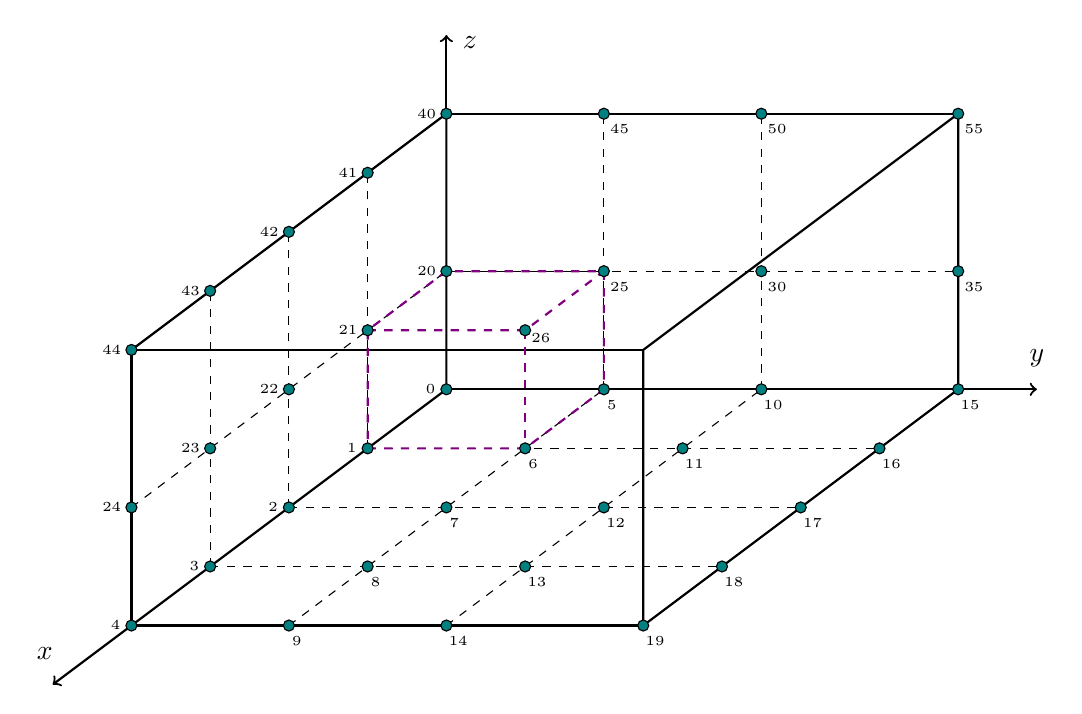
\begin{tikzpicture}
%\draw[step=0.5cm,gray,very thin] (0,0) grid (14,10); %background grid

%element
\draw[thick] (2,2) -- (8.5,2) -- (8.5,5.5) -- (2,5.5) -- cycle;  
\draw[thick] (2,2) -- (6,5) -- (6,8.5) -- (2,5.5) -- cycle ;
\draw[thick] (8.5,2) -- (12.5,5) -- (12.5,8.5) -- (8.5,5.5) -- cycle ;
\draw[thick] (6,5) -- (12.5,5) ;
\draw[thick] (6,8.5) -- (12.5,8.5) ;

%axes
\draw[thick,->] (2,2)--(1,1.25);
\draw[thick,->] (12.5,5)--(13.5,5);
\draw[thick,->] (6,8.5)--(6,9.5);
\node[] at (0.9,1.65) {$x$};
\node[] at (13.5,5.4) {$y$};
\node[] at (6.3,9.4) {$z$};

\draw[dashed] (2,3.5)--(6,6.5);
\draw[dashed] (3,2.75)--(3,6.25);
\draw[dashed] (4,3.5)--(4,7);
\draw[dashed] (5,4.25)--(5,7.75);
\draw[dashed] (4,2)--(8,5);
\draw[dashed] (6,2)--(10,5);
\draw[dashed] (3,2.75)--(9.5,2.75);
\draw[dashed] (4,3.5)--(10.5,3.5);
\draw[dashed] (5,4.25)--(11.5,4.25);
\draw[dashed] (6,6.5)--(12.5,6.5);
\draw[dashed] (8,5)--(8,8.5);
\draw[dashed] (10,5)--(10,8.5);

\draw[dashed, thick,violet] (5,4.25)--(7,4.25) --(8,5)--(8,6.5) --(6,6.5)--(5,5.75)--(5,4.25);
\draw[dashed, thick,violet] (5,5.75)--(7,5.75)--(8,6.5);
\draw[dashed, thick,violet] (7,5.75)--(7,4.25);

\draw[black,fill=teal] (2,2) circle (2pt); 
\draw[black,fill=teal] (3,2.75) circle (2pt); 
\draw[black,fill=teal] (4,3.5) circle (2pt); 
\draw[black,fill=teal] (5,4.25) circle (2pt); 
\draw[black,fill=teal] (6,5) circle (2pt); 

\draw[black,fill=teal] (2,3.5) circle (2pt); 
\draw[black,fill=teal] (3,4.25) circle (2pt); 
\draw[black,fill=teal] (4,5) circle (2pt); 
\draw[black,fill=teal] (5,5.75) circle (2pt); 
\draw[black,fill=teal] (6,6.5) circle (2pt); 

\draw[black,fill=teal] (2,5.5) circle (2pt); 
\draw[black,fill=teal] (3,6.25) circle (2pt); 
\draw[black,fill=teal] (4,7) circle (2pt); 
\draw[black,fill=teal] (5,7.75) circle (2pt); 
\draw[black,fill=teal] (6,8.5) circle (2pt); 

\draw[black,fill=teal] (4,2) circle (2pt); 
\draw[black,fill=teal] (5,2.75) circle (2pt); 
\draw[black,fill=teal] (6,3.5) circle (2pt); 
\draw[black,fill=teal] (7,4.25) circle (2pt); 
\draw[black,fill=teal] (8,5) circle (2pt); 

\draw[black,fill=teal] (6,2) circle (2pt); 
\draw[black,fill=teal] (7,2.75) circle (2pt); 
\draw[black,fill=teal] (8,3.5) circle (2pt); 
\draw[black,fill=teal] (9,4.25) circle (2pt); 
\draw[black,fill=teal] (10,5) circle (2pt); 

\draw[black,fill=teal] (8.5,2) circle (2pt); 
\draw[black,fill=teal] (9.5,2.75) circle (2pt); 
\draw[black,fill=teal] (10.5,3.5) circle (2pt); 
\draw[black,fill=teal] (11.5,4.25) circle (2pt); 
\draw[black,fill=teal] (12.5,5) circle (2pt);

\draw[black,fill=teal] (7,5.75) circle (2pt);


\draw[black,fill=teal] (8,6.5) circle (2pt);
\draw[black,fill=teal] (8,8.5) circle (2pt);

\draw[black,fill=teal] (10,6.5) circle (2pt);
\draw[black,fill=teal] (10,8.5) circle (2pt);

\draw[black,fill=teal] (12.5,6.5) circle (2pt);
\draw[black,fill=teal] (12.5,8.5) circle (2pt);

\node[] at (5.8,5) {\tiny 0};
\node[] at (4.8,4.25) {\tiny 1};
\node[] at (3.8,3.5) {\tiny 2};
\node[] at (2.8,2.75) {\tiny 3};
\node[] at (1.8,2) {\tiny 4};

\node[] at (5.75,6.5) {\tiny 20};
\node[] at (4.75,5.75) {\tiny 21};
\node[] at (3.75,5) {\tiny 22};
\node[] at (2.75,4.25) {\tiny 23};
\node[] at (1.75,3.5) {\tiny 24};

\node[] at (5.75,8.5) {\tiny 40};
\node[] at (4.75,7.75) {\tiny 41};
\node[] at (3.75,7) {\tiny 42};
\node[] at (2.75,6.25) {\tiny 43};
\node[] at (1.75,5.5) {\tiny 44};

\node[] at (8.1,4.8) {\tiny 5};
\node[] at (7.1,4.05) {\tiny 6};
\node[] at (6.1,3.3) {\tiny 7};
\node[] at (5.1,2.55) {\tiny 8};
\node[] at (4.1,1.8) {\tiny 9};

\node[] at (10.15,4.8) {\tiny 10};
\node[] at (9.15,4.05) {\tiny 11};
\node[] at (8.15,3.3) {\tiny 12};
\node[] at (7.15,2.55) {\tiny 13};
\node[] at (6.15,1.8) {\tiny 14};

\node[] at (12.65,4.8) {\tiny 15};
\node[] at (11.65,4.05) {\tiny 16};
\node[] at (10.65,3.3) {\tiny 17};
\node[] at (9.65,2.55) {\tiny 18};
\node[] at (8.65,1.8) {\tiny 19};

\node[] at (8.2,6.3) {\tiny 25};
\node[] at (7.2,5.65) {\tiny 26};

\node[] at (8.2,8.3) {\tiny 45};
\node[] at (10.2,6.3) {\tiny 30};
\node[] at (10.2,8.3) {\tiny 50};

\node[] at (12.7,6.3) {\tiny 35};
\node[] at (12.7,8.3) {\tiny 55};

\end{tikzpicture}

\end{center}



The total number of nonzeros in the case $ndof=1$ would be decomposed as follows:
\begin{itemize}
\item 8 corners 'see' 8 neighbours
\item 4 edges with $(nnx-2)$ nodes in the x direction see 12 nodes
\item 4 edges with $(nny-2)$ nodes in the y direction see 12 nodes
\item 4 edges with $(nnz-2)$ nodes in the z direction see 12 nodes
\item $2(nnx-2)(nny-2)$ nodes see 18 nodes
\item $2(nnx-2)(nnz-2)$ nodes see 18 nodes
\item $2(nny-2)(nnz-2)$ nodes see 18 nodes
\item $(nnx-2)(nny-2)(nnz-2)$ interior nodes see 27 nodes
\end{itemize}

%..............................................................................
\subsubsection{3D domain - CSR- Q2 - one degree of freedom}


\begin{center}
\begin{flushright} {\tiny {\color{gray} (tikz\_4x3x2\_q2.tex)}} \end{flushright}
%~~~~~~~~~~~~~~~~~~~~~~~~~~~~~~~~~~~~~~~~~~~~~~~~~~~~~~~~~~~~~~~~~~~~~~~~~~~~~~~~~~~~~~~~~~~~~~~~~~

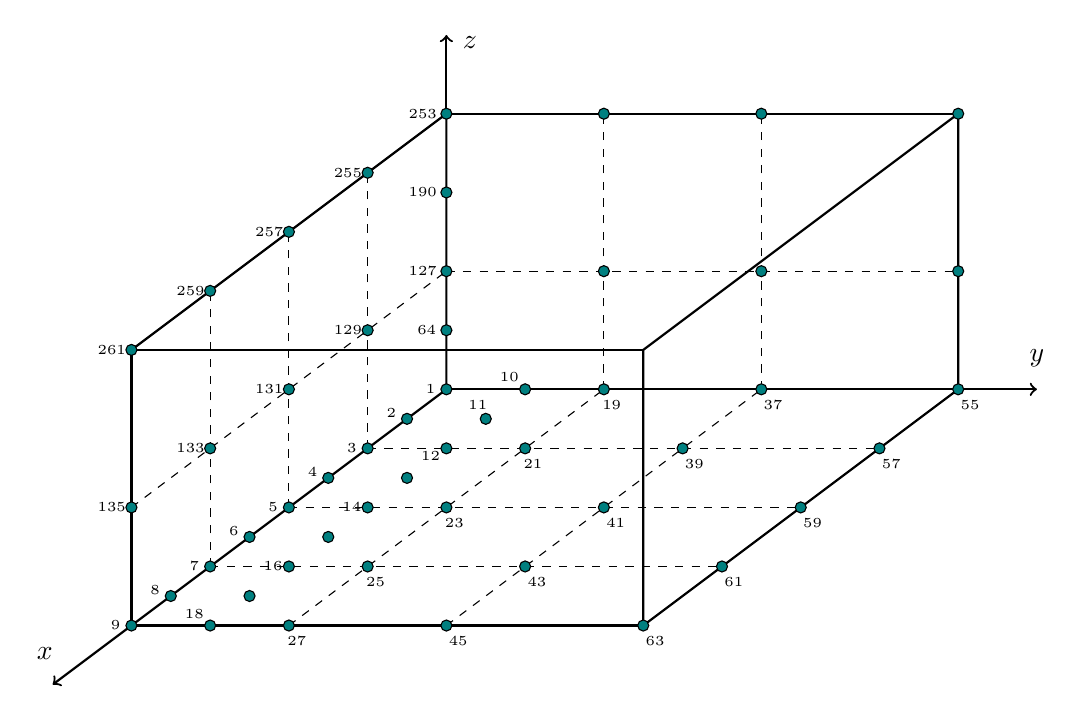
\begin{tikzpicture}
%\draw[step=0.5cm,gray,very thin] (0,0) grid (14,10); %background grid

%element
\draw[thick] (2,2) -- (8.5,2) -- (8.5,5.5) -- (2,5.5) -- cycle;  
\draw[thick] (2,2) -- (6,5) -- (6,8.5) -- (2,5.5) -- cycle ;
\draw[thick] (8.5,2) -- (12.5,5) -- (12.5,8.5) -- (8.5,5.5) -- cycle ;
\draw[thick] (6,5) -- (12.5,5) ;
\draw[thick] (6,8.5) -- (12.5,8.5) ;

%axes
\draw[thick,->] (2,2)--(1,1.25);
\draw[thick,->] (12.5,5)--(13.5,5);
\draw[thick,->] (6,8.5)--(6,9.5);
\node[] at (0.9,1.65) {$x$};
\node[] at (13.5,5.4) {$y$};
\node[] at (6.3,9.4) {$z$};

\draw[dashed] (2,3.5)--(6,6.5);
\draw[dashed] (3,2.75)--(3,6.25);
\draw[dashed] (4,3.5)--(4,7);
\draw[dashed] (5,4.25)--(5,7.75);
\draw[dashed] (4,2)--(8,5);
\draw[dashed] (6,2)--(10,5);
\draw[dashed] (3,2.75)--(9.5,2.75);
\draw[dashed] (4,3.5)--(10.5,3.5);
\draw[dashed] (5,4.25)--(11.5,4.25);
\draw[dashed] (6,6.5)--(12.5,6.5);
\draw[dashed] (8,5)--(8,8.5);
\draw[dashed] (10,5)--(10,8.5);


\draw[black,fill=teal] (2,2) circle (2pt);  %9
\draw[black,fill=teal] (2.5,2.375) circle (2pt); 
\draw[black,fill=teal] (3,2.75) circle (2pt); 
\draw[black,fill=teal] (3.5,3.125) circle (2pt); 
\draw[black,fill=teal] (4,3.5) circle (2pt); 
\draw[black,fill=teal] (4.5,3.875) circle (2pt); 
\draw[black,fill=teal] (5,4.25) circle (2pt); 
\draw[black,fill=teal] (5.5,4.625) circle (2pt); 
\draw[black,fill=teal] (6,5) circle (2pt);  % 1

\draw[black,fill=teal] (3,2) circle (2pt);  %18
\draw[black,fill=teal] (3.5,2.375) circle (2pt); 
\draw[black,fill=teal] (4,2.75) circle (2pt); 
\draw[black,fill=teal] (4.5,3.125) circle (2pt); 
\draw[black,fill=teal] (5,3.5) circle (2pt); 
\draw[black,fill=teal] (5.5,3.875) circle (2pt); 
\draw[black,fill=teal] (6,4.25) circle (2pt); 
\draw[black,fill=teal] (6.5,4.625) circle (2pt); 
\draw[black,fill=teal] (7,5) circle (2pt);  % 10



\draw[black,fill=teal] (2,3.5) circle (2pt); 
\draw[black,fill=teal] (3,4.25) circle (2pt); 
\draw[black,fill=teal] (4,5) circle (2pt); 
\draw[black,fill=teal] (5,5.75) circle (2pt); 
\draw[black,fill=teal] (6,6.5) circle (2pt); 

\draw[black,fill=teal] (2,5.5) circle (2pt); 
\draw[black,fill=teal] (3,6.25) circle (2pt); 
\draw[black,fill=teal] (4,7) circle (2pt); 
\draw[black,fill=teal] (5,7.75) circle (2pt); 
\draw[black,fill=teal] (6,8.5) circle (2pt); 

\draw[black,fill=teal] (4,2) circle (2pt); 
\draw[black,fill=teal] (5,2.75) circle (2pt); 
\draw[black,fill=teal] (6,3.5) circle (2pt); 
\draw[black,fill=teal] (7,4.25) circle (2pt); 
\draw[black,fill=teal] (8,5) circle (2pt); 

\draw[black,fill=teal] (6,2) circle (2pt); 
\draw[black,fill=teal] (7,2.75) circle (2pt); 
\draw[black,fill=teal] (8,3.5) circle (2pt); 
\draw[black,fill=teal] (9,4.25) circle (2pt); 
\draw[black,fill=teal] (10,5) circle (2pt); 

\draw[black,fill=teal] (8.5,2) circle (2pt); 
\draw[black,fill=teal] (9.5,2.75) circle (2pt); 
\draw[black,fill=teal] (10.5,3.5) circle (2pt); 
\draw[black,fill=teal] (11.5,4.25) circle (2pt); 
\draw[black,fill=teal] (12.5,5) circle (2pt);

\draw[black,fill=teal] (6,5.75) circle (2pt); %64
\draw[black,fill=teal] (6,7.5) circle (2pt); %190

\draw[black,fill=teal] (8,6.5) circle (2pt);
\draw[black,fill=teal] (8,8.5) circle (2pt);

\draw[black,fill=teal] (10,6.5) circle (2pt);
\draw[black,fill=teal] (10,8.5) circle (2pt);

\draw[black,fill=teal] (12.5,6.5) circle (2pt);
\draw[black,fill=teal] (12.5,8.5) circle (2pt);

\node[] at (5.8,5) {\tiny 1};
\node[] at (5.3,4.7) {\tiny 2};
\node[] at (4.8,4.25) {\tiny 3};
\node[] at (4.3,3.95) {\tiny 4};
\node[] at (3.8,3.5) {\tiny 5};
\node[] at (3.3,3.2) {\tiny 6};
\node[] at (2.8,2.75) {\tiny 7};
\node[] at (2.3,2.45) {\tiny 8};
\node[] at (1.8,2) {\tiny 9};

\node[] at (6.8,5.15) {\tiny 10};
\node[] at (6.4,4.8) {\tiny 11};
\node[] at (5.8,4.15) {\tiny 12};
\node[] at (4.8,3.5) {\tiny 14};
\node[] at (3.8,2.75) {\tiny 16};
\node[] at (2.8,2.15) {\tiny 18};

\node[] at (8.1,4.8) {\tiny 19};
\node[] at (7.1,4.05) {\tiny 21};
\node[] at (6.1,3.3) {\tiny 23};
\node[] at (5.1,2.55) {\tiny 25};
\node[] at (4.1,1.8) {\tiny 27};

\node[] at (10.15,4.8) {\tiny 37};
\node[] at (9.15,4.05) {\tiny 39};
\node[] at (8.15,3.3) {\tiny 41};
\node[] at (7.15,2.55) {\tiny 43};
\node[] at (6.15,1.8) {\tiny 45};

\node[] at (12.65,4.8) {\tiny 55};
\node[] at (11.65,4.05) {\tiny 57};
\node[] at (10.65,3.3) {\tiny 59};
\node[] at (9.65,2.55) {\tiny 61};
\node[] at (8.65,1.8) {\tiny 63};

\node[] at (5.75,5.75) {\tiny 64};

\node[] at (5.7,6.5) {\tiny 127};
\node[] at (4.75,5.75) {\tiny 129};
\node[] at (3.75,5) {\tiny 131};
\node[] at (2.75,4.25) {\tiny 133};
\node[] at (1.75,3.5) {\tiny 135};

\node[] at (5.7,7.5) {\tiny 190};

\node[] at (5.7,8.5) {\tiny 253};
\node[] at (4.75,7.75) {\tiny 255};
\node[] at (3.75,7) {\tiny 257};
\node[] at (2.75,6.25) {\tiny 259};
\node[] at (1.75,5.5) {\tiny 261};

\end{tikzpicture}


\end{center}





%..............................................................................
\subsubsection{Matrix Storage in fieldstone}

The majority of the codes have the FE matrix being a full array
\begin{lstlisting}
a_mat = np.zeros((Nfem,Nfem),dtype=np.float64) 
\end{lstlisting}
and it is converted to CSR format on the fly in the solve phase:
\begin{lstlisting}
sol = sps.linalg.spsolve(sps.csr_matrix(a_mat),rhs)
\end{lstlisting}

Note that linked list storages can be used (lil\_matrix). Substantial memory savings 
but much longer compute times since it takes longer to write in such arrays.
A conversion to CSR format is still necessary before calling the solver.




%..............................................................................
\subsubsection{About Sparse Matrix-Vector multiplication} \label{ss:spmv}
\index{general}{SpMV} \index{general}{Sparse Matrix-Vector Multiplication}

When/if the matrix ${\bm M}$ is stored in a two-dimensional array, 
its (left or right) multiplication by a vector is trivial. 
Either one resorts to writing a double for loop (not recommended), 
either one uses {\tt numpy.dot}\footnote{\url{https://numpy.org/doc/stable/reference/generated/numpy.dot.html}}
in python, or {\tt matmul} in Fortran.

However, when the matrix is stored as a single continuous array, say CSR, how does this work?
This question is {\it very important} since iterative solvers such as the Conjugate Gradient solver
(see Section~\ref{ss:itsolvers}) rely extensively on multiplying the matrix by many different vectors. 

The Sparse Matrix-Vector multiplication operation is often abbreviated SpMV.
To quote Knepley \cite{knepley}: "The Sparse Matrix-Vector Product (SpMV) is today 
a workhorse of scientific computing. It is a central kernel is iterative linear and 
nonlinear solvers for PDE, and now for many graph algorithms."
As explained in Williams \etal (2007) \cite{wiov07} (and in many 
other sources on the topic), the algorithm for 
a basic SpMV implementation is rather simple in its naive form. 

\begin{center}
\includegraphics[width=17cm]{images/spmv/widc08}\\
{\captionfont Taken from Williams \etal (2008) \cite{widc08}. 
Sparse Matrix Vector Multiplication (SpMV). 
(a) visualization of the algebra: $\vec{y} \leftarrow {\bm A}\cdot \vec{x}$.\\
(b) Standard compressed sparse row (CSR) representation of the matrix.  \\
(c) The standard implementation of SpMV for a matrix stored in CSR. 
The outer loop is trivially parallelized without any data dependencies.}
\end{center}

Let us assume that we wish to compute $\vec{y}={\bm A}\cdot \vec{x}$ where ${\bm A}$ 
is in CSR format. The pseudo code then goes as follows:
\begin{verbatim}
for i in range(0,m):
    y0=0
    for k in range(ROWPTR[i],ROWPTR[i+1]):
        y0 += VAL[k] * x[COLIND[k]]
    y[i]=y0
\end{verbatim} 
Although technically correct, this algorithm is problematic because the vector x array
is accessed indirectly and this causes a non-optimal use of the processor, which 
in the end makes the calculation take longer than it should.


The following piece of code comes from \elefant. Note that here (ROWPTR=ia, COLIND=ja, VAL=mat)
\begin{lstlisting}[language=Fortran]
subroutine spmv (nr,nc,nz,x,y,mat,ja,ia)
implicit none
integer, intent(in)  :: nr,nc,nz
real(8), intent(in)  :: x(nc), mat(nz)
real(8), intent(out) :: y(nr)
integer, intent(in)  :: ja(nz),ia(nr+1)
real(8) t
integer i, k

do i = 1,nr
   t = 0.0d0
   do k=ia(i), ia(i+1)-1
      t = t + mat(k)*x(ja(k))
   end do
   y(i) = t 
end do

end subroutine
\end{lstlisting}


How to make this calculation as efficiently as possible on CPUs and GPUs, on one thread 
or multiple threads has given rise to a lot of literature.

\Literature Krotkiewski \& Dabrowski \cite{krda10}, Section 9.4 of Kepley \cite{knepley}, 
Williams \etal (2008) \cite{widc08}

%..............................................................................
\subsubsection{SpMV and SpMV-T with the CSR format - a concrete example}

(What follows was orignally written for \elefant so that code excerpts and loop indexing 
are those of Fortran.)

Let us consider a simple matrix $\mathbb{G}$ which is not square (size is $3\times5$):
\[
\G^T=
\left(
\begin{array}{ccccc}
{\color{teal} 1} & {\color{teal}0}& {\color{teal}4}& {\color{teal}1}& {\color{teal}2}\\
{\color{violet}0}& {\color{violet}1}& {\color{violet}1}& {\color{violet}1}& {\color{violet}0}\\
{\color{orange}3}& {\color{orange}0} & {\color{orange}0}& {\color{orange}7}& {\color{orange}1}
\end{array}
\right)
\]

The number of rows is $nr=3$, the number of columns is $nc=5$ and the number of nonzeros is 
$nz=10$.

Let us consider two vectors $\vec{\cal V}^T=(1,1,1,1,1)$ and $\vec{\cal P}^T=(1,1,1)$.
Obviously, we have:
\[
{\G}^T \cdot \vec{\cal V} = 
\left(
\begin{array}{c}
8\\3\\11
\end{array}
\right)
\qquad
\text{and}
\qquad
{\G} \cdot \vec{\cal P} = 
\left(
\begin{array}{c}
4 \\ 1\\ 5\\ 9\\ 3
\end{array}
\right)
\]

The CSR storage of ${\G}^T$ requires three arrays:
$ia$ (integer, size $nr+1$), $ja$ (integer, size $nz$) and $mat$ (real, size $nz$). 
In the case of the small matrix above:
\begin{eqnarray}
ia &=&(1,5,8,11)  \nn\\
ja &=&(1,3,4,5,2,3,4,1,4,5) \nn\\
mat&=&({\color{teal} 1,4,1,2},{\color{violet}1,1,1},{\color{orange}3,7,1}) \nn
\end{eqnarray}
The sparse matrix vector multiplication kernel SpMV for $\vec{y} = {\bm A}\cdot \vec{x}$ 
has been explained above, and it is trivial to carry out this algorithm by hand 
and verify that the vector $y$ is given by $y^T=(8,3,11)$.

Let us now turn to an interesting problem. Is it possible with the same arrays $ia,ja,mat$ to compute the 
multiplication of the transpose of the matrix with a vector? 
The answer is of course positive and the code is given hereunder:

\begin{lstlisting}[language=Fortran]
y=0.d0
do i = 1,nr
   do k=ia(i), ia(i+1)-1
      y(ja(k))=y(ja(k))+mat(k)*x(i)
   end do
end do
\end{lstlisting}

Let us take $i=1$. The variable $k$ then goes from 1 to 4. 
The inner loop does:
\begin{verbatim}
y(1)=y(1)+mat(1)*x(1)
y(3)=y(3)+mat(2)*x(1)
y(4)=y(4)+mat(3)*x(1)
y(5)=y(5)+mat(4)*x(1)
\end{verbatim}

Let us take $i=2$. The variable $k$ then goes from 5 to 7. 
The inner loop does:
\begin{verbatim}
y(2)=y(2)+mat(5)*x(2)
y(3)=y(3)+mat(6)*x(2)
y(4)=y(4)+mat(7)*x(2)
\end{verbatim}

Let us take $i=3$. The variable $k$ then goes from 8 to 10. 
The inner loop does:
\begin{verbatim}
y(1)=y(1)+mat(8)*x(3)
y(4)=y(4)+mat(9)*x(3)
y(5)=y(5)+mat(10)*x(3)
\end{verbatim}

So in total, we have:
\begin{verbatim}
y(1)=mat(1)*x(1)+mat(8)*x(3)
y(2)=mat(5)*x(2)
y(3)=mat(2)*x(1)+mat(6)*x(2)
y(4)=mat(3)*x(1)+mat(7)*x(2)+mat(9)*x(3)
y(5)=mat(4)*x(1)+mat(10)*x(3)
\end{verbatim}
which is indeed the result of the transposed of the matrix multiplied by a vector $\vec{x}$.

\vspace{0.6cm}

Let us consider a simple matrix $\K$ which is square (size is $5\times5$):
\[
\K=
\left(
\begin{array}{ccccc}
1&0&4&1&2\\
0&1&0&1&0\\
4&0&0&7&1\\
1&1&7&4&0\\
2&0&1&0&5
\end{array}
\right)
\]

In this case , NZ=16.
\begin{eqnarray}
ia &=&(1,5,7,10,14,17) \nn\\
ja &=&(1,3,4,5,\;\; 2,4, \;\; 1,4,5, \;\; 1,2,3,4, \;\; 1,3,5) \nn\\
mat&=&(1,4,1,2,1,1,4,7,1,1,1,7,4,2,1,5) \nn
\end{eqnarray}
The sparse matrix vector multiplication kernel SpMV for $\vec{y} = {\bm A}\cdot \vec{x}$ 
is given  as follows in its simplest form.
Since the matrix is symmetric, there is no use to store the whole matrix. Its upper half (for instance) will do. 
In this case, NZ=
and then 
\begin{eqnarray}
ia &=&(1,5,7,9,10,11) \nn\\
ja &=&(1,3,4,5,\;\; 2,4, \;\; 4,5, \;\; 4, \;\; 5) \nn\\
mat&=&(1,4,1,2,\;\; 1,1, \;\; 7,1, \;\; 4,\;\; 5) \nn
\end{eqnarray}

All is good and well until one wishes to multiply the real matrix by a vector. 
The SpMV routines described above will not work since it will return the upper half of the matrix 
multiplied by the vector.

One can then write a decicated algorithm:
\begin{verbatim}
do i = 1,nr

   ! multiply the upper half by the vector

   do k=ia(i), ia(i+1)-1
      y(i) = y(i) + mat(k)*x(ja(k))
   end do

   ! multiply the transpose of matrix by vector
   ! but omit diagonal 

   do k=ia(i), ia(i+1)-1
      if (i/=ja(k)) then
         y(ja(k))=y(ja(k))+mat(k)*x(i)
      end if
   end do

end do
\end{verbatim}


Example:

\begin{verbatim}
y(1)
=y(1) + mat(1)*x(ja(1)) + mat(2)*x(ja(2)) + mat(3)*x(ja(3)) + mat(4)*x(ja(4)) 
=y(1) + mat(1)*x(1) + mat(2)*x(3) + mat(3)*x(4) + mat(4)*x(5) 
\end{verbatim}
etc ...

Finish?

 




